\graphicspath{{images/fake_rate}}

\section{Fake Rate}\label{sec:fake_rate}
For this analysis, there are two backgrounds that are estimated by a fake rate method, nonprompt and charge misId. Because the signal region contains two same-sign leptons, the larger background samples are suppressed significantly, such as Drell-Yan and ttbar (or samples listed in~\ref{tab:signal_xsec} under Other). While our selection removes these samples, non-trivial fake rates couple with these large sample's cross-sections lead to many fake events coming from these large backgrounds. Often, these fake are poorly modeled in MC and require scale factors to fix and are statistics limited since they have a small yield in a large cross-section sample.

To alleviate this, fake rates are measured in data and applied to a side band region to transfer to our signal region. By measuring the fake rate in data, the rate is not subject to usual systematics associated with MC, and by transferring events, the statistics are much better since the yield is artificially lowered by the fake rates which are used as transfer factors.

Following is a description of the process for these fake rates

\subsection{Nonprompt Lepton}\label{sec:nonprompt_lepton}

\subsubsection{Overview}\label{sec:nonprompt:overview}
Nonprompt Leptons are defined as leptons not originating from the main process, but rather are produced outside of the main tree level feynman diagram. Usually these leptons come from decays of jets. Because they are produced from jets, we remove a majority by applying a isolation cut which limits the relative jet energy close to the lepton. To further remove nonprompt leptons, the TTH Group developed an MVA specifically to categorize prompt leptons from nonprompt leptons, and for this analysis, the definition of our tight leptons is by a cut at 0.4 on the TTH MVA.\@ While this would normally remove most nonprompt leptons, our Same-Sign requirement reduces the yield of samples with large cross-sections and single lepton or OS signatures making the proportion of nonprompt leptons non-trivial. Because of this, we expect most nonprompt leptons to come from DY, ttbar, and W+Jets.

To measure this fake rate, we measure in a QCD multijet region which is enriched in jets that fake tight, prompt leptons. To have as pure of a QCD sample, we use a region with low MET and low $M_{T}$. For the measurement process, to reduce influence of systematic errors, we also measure the fake rate using data. For getting a proper fake rate, we need to subtract the prompt contamination in our QCD measurement region which is done by subtracting EWK MC from the data. To get the correct normalization for the EWK MC, we fit it to a sideband region defined by inverting the MET cut on the measurement region. Because our signal region is primarily made up of ttbar and we expect a majority of the fakes to be coming from that, we also have to worry about the amount of fakes coming from bjets. To regulate this, we require a recoiling btagged jet in our QCD measurement region to match what we expect to see in our signal region.

After this fake rate is measured, we can then test it in a closure region. For this, we use a signal-like region where some of the cuts have been relaxed to allow for higher statistics in our Nonprompt background. This closure test is used to estimate the error in the data-driven nonprompt background. We use a simple log-normal systematic error based on the error we see in our closure region for applying the error in our fit model.

% \subsubsection{Trigger Efficiency}
% For our fake rate measurement, we look at a QCD multijet region with 1 lepton and 1 recoiling jet. Because of the $\pt$ requirements of our leptons, we must consider a low $\pt$ trigger. Further, our method uses a correction on the fake lepton $\pt$ that can allow for leptons with $\pt < 15\gev$ which is our tight lepton threshold. Because of this, we use the highly prescaled, single lepton triggers listed in~\ref{tab:triggers}.

% The trigger are applied based on the $\pt$ range the lepton falls into as shown bellow:
% \begin{itemize}
%   \item $\pt(\mu) < 20\gev$: Mu8
%   \item $\pt(\mu) > 20\gev$: Mu17
%   \item $\pt(e) < 25\gev$: Ele12
%   \item $\pt(e) < 25\gev$: Ele23
% \end{itemize}
% This means we use the lower-pt trigger (Mu8 and Ele12) with only lower $\pt$ leptons and vice-versa for the high-pt triggers (Mu17 and Ele23). We thus can look at the $\pt$ spectrum around the turn on for all 4 of our triggers to see where our $\pt$ threshold has to be to be in the plateau:

% \begin{figure}
%   \centering
%   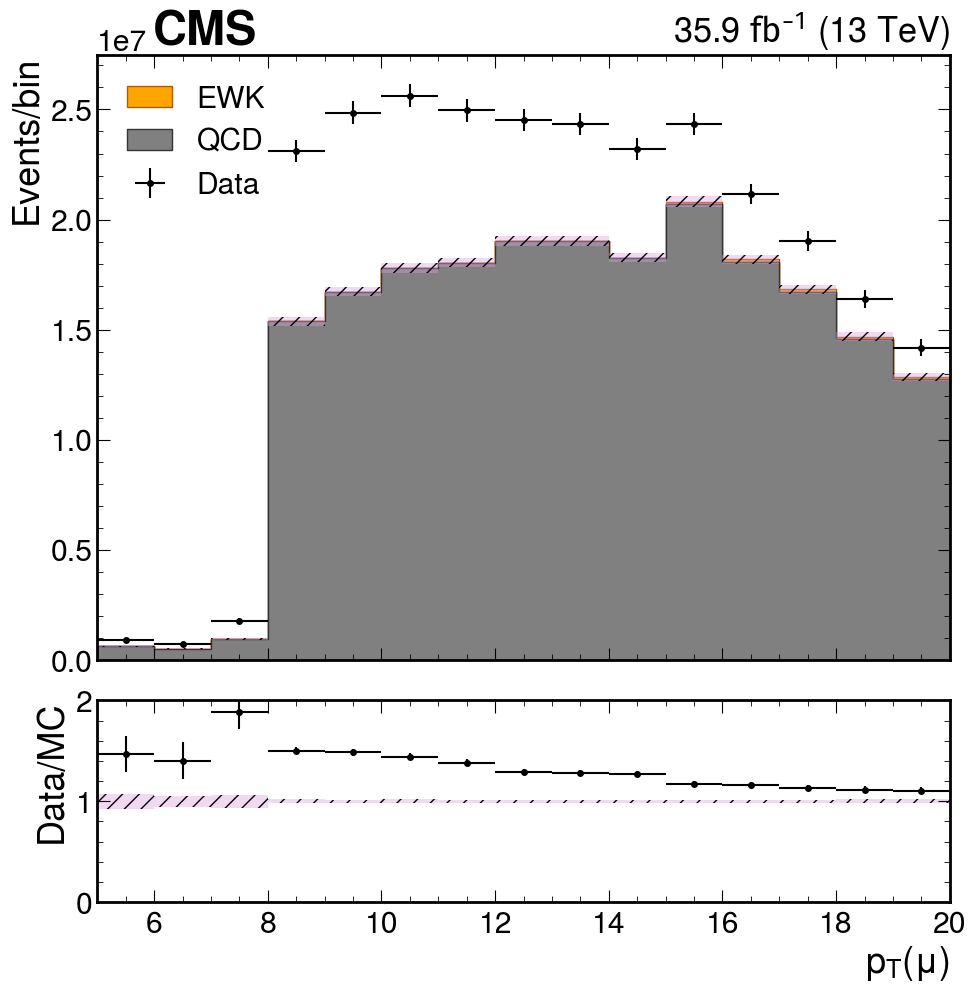
\includegraphics[width=0.4\textwidth]{images/fake_rate/trigger_eff/rawpt_low_Muon_2016.png}
%   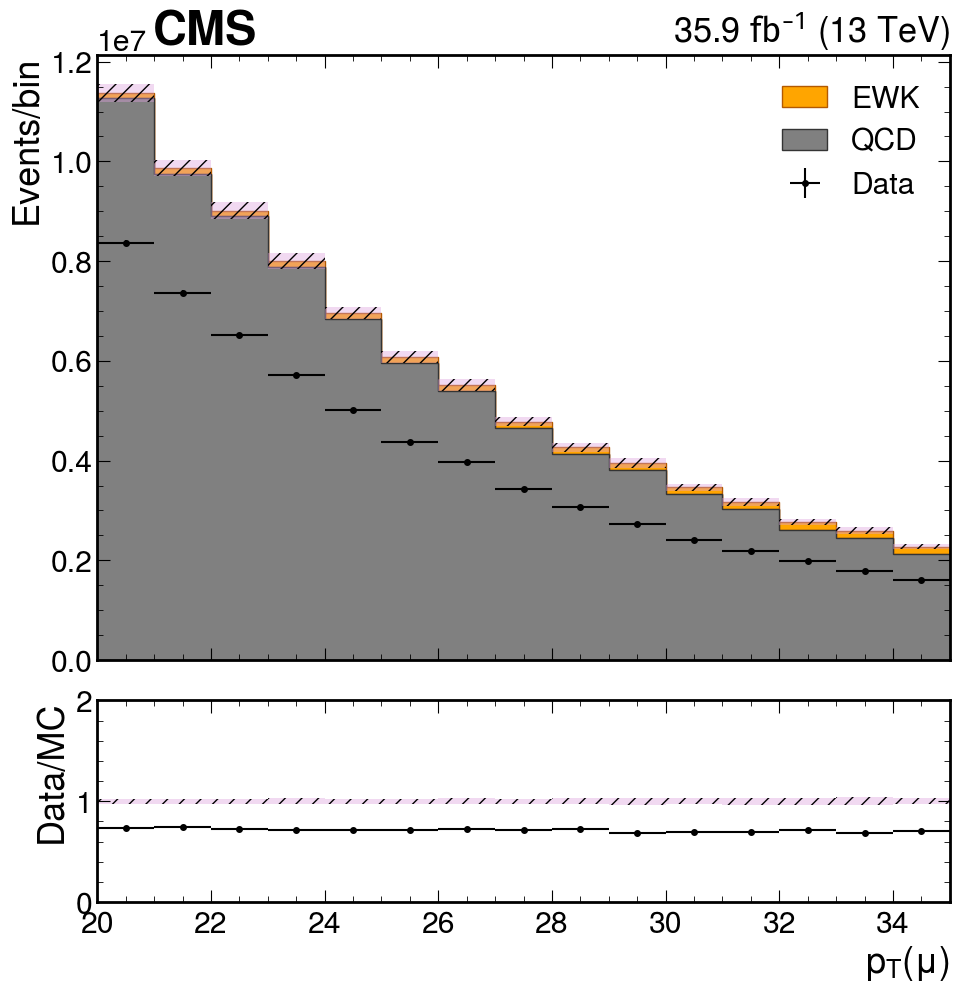
\includegraphics[width=0.4\textwidth]{images/fake_rate/trigger_eff/rawpt_high_Muon_2016.png}\\
%   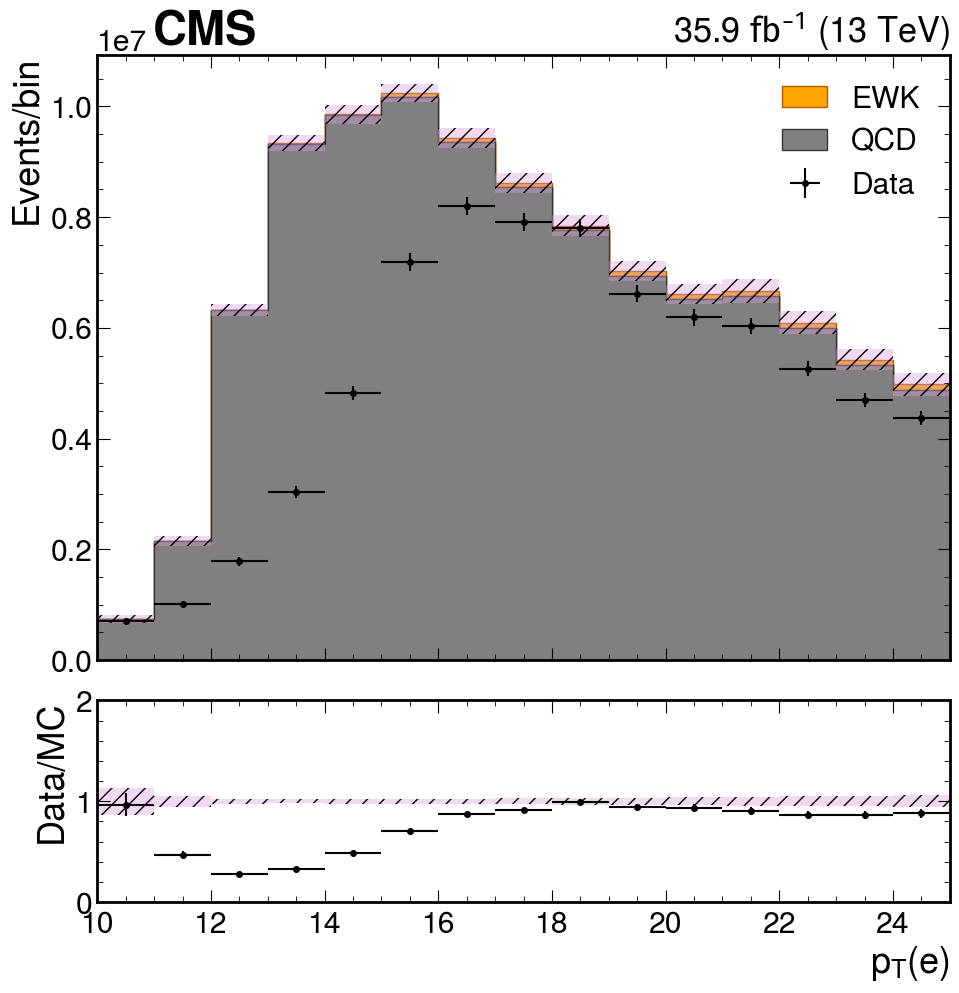
\includegraphics[width=0.4\textwidth]{images/fake_rate/trigger_eff/rawpt_low_Electron_2016.png}
%   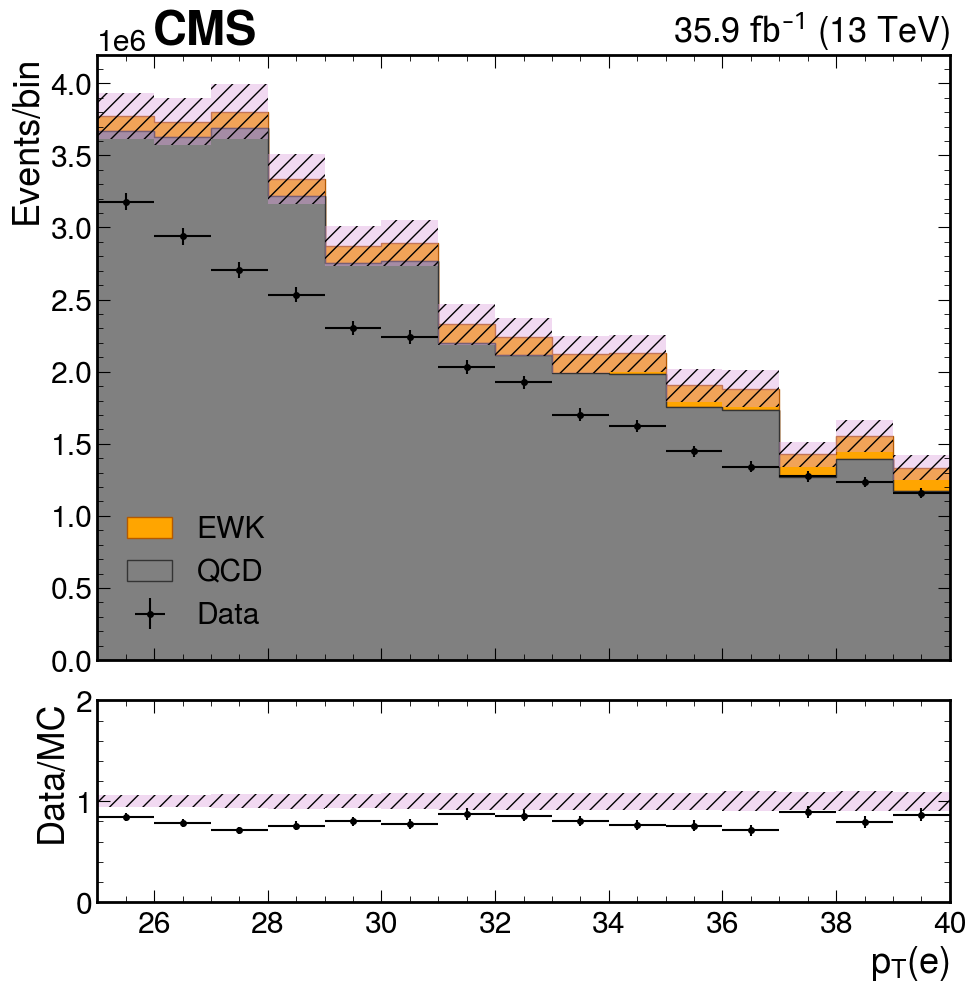
\includegraphics[width=0.4\textwidth]{images/fake_rate/trigger_eff/rawpt_high_Electron_2016.png}\\
%   \caption{Trigger turn-on curves for 2016. Left shows low-pt trigger, right show high-pt trigger. Top shows muons, Bottom Electrons.}\label{fig:2016_trigger_turnon}
% \end{figure}


% \begin{figure}
%   \centering
%   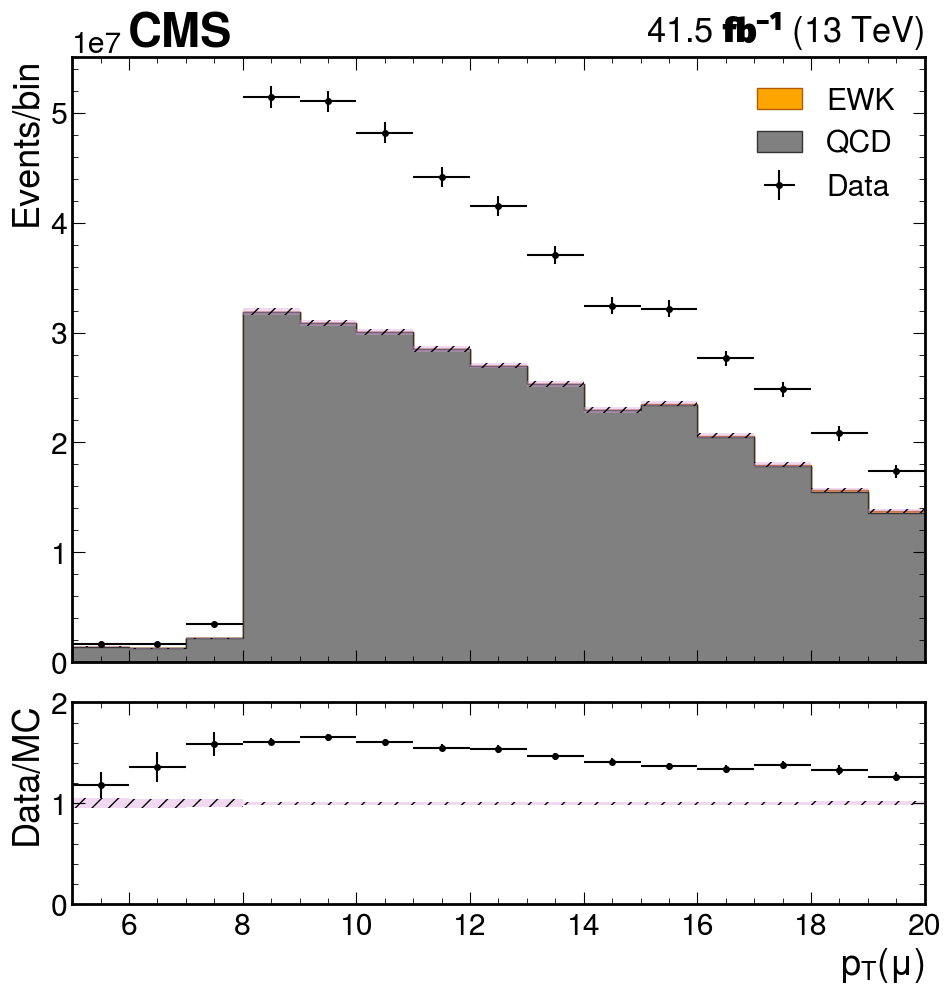
\includegraphics[width=0.45\textwidth]{images/fake_rate/trigger_eff/rawpt_low_Muon_2017.png} \hfill
%   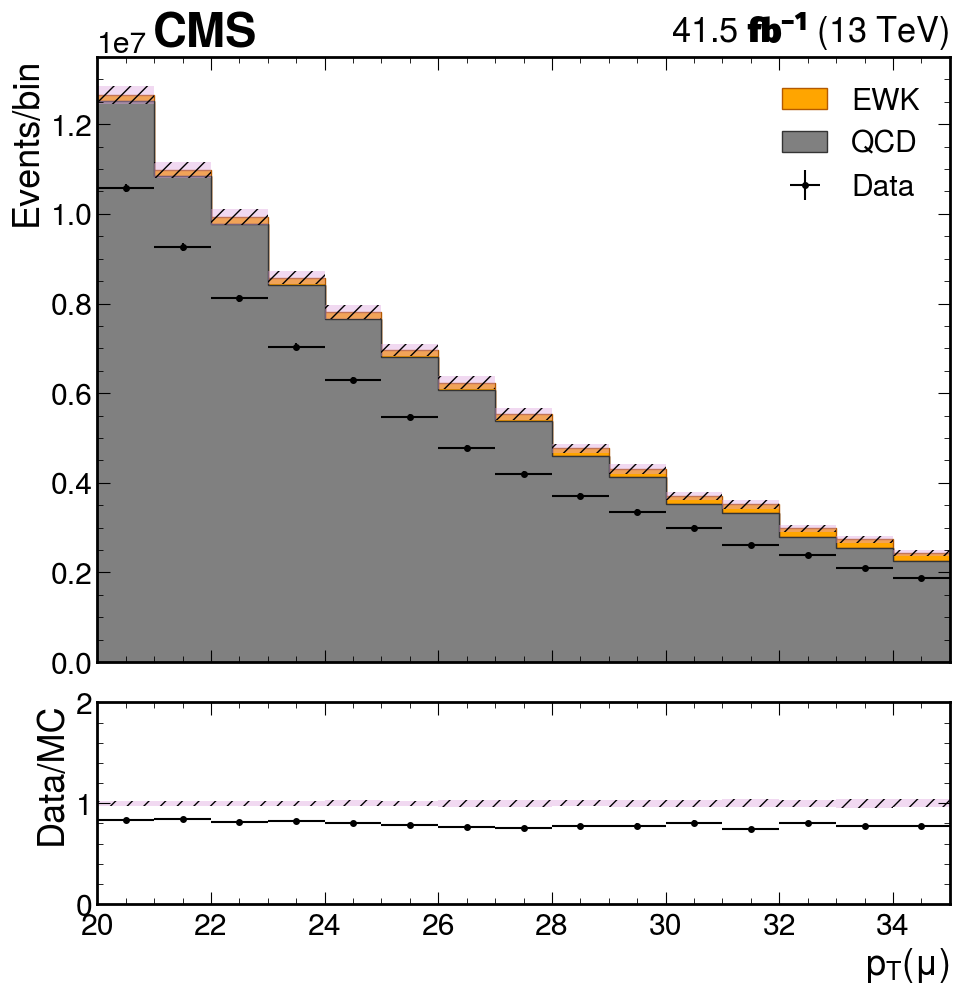
\includegraphics[width=0.45\textwidth]{images/fake_rate/trigger_eff/rawpt_high_Muon_2017.png}\\
%   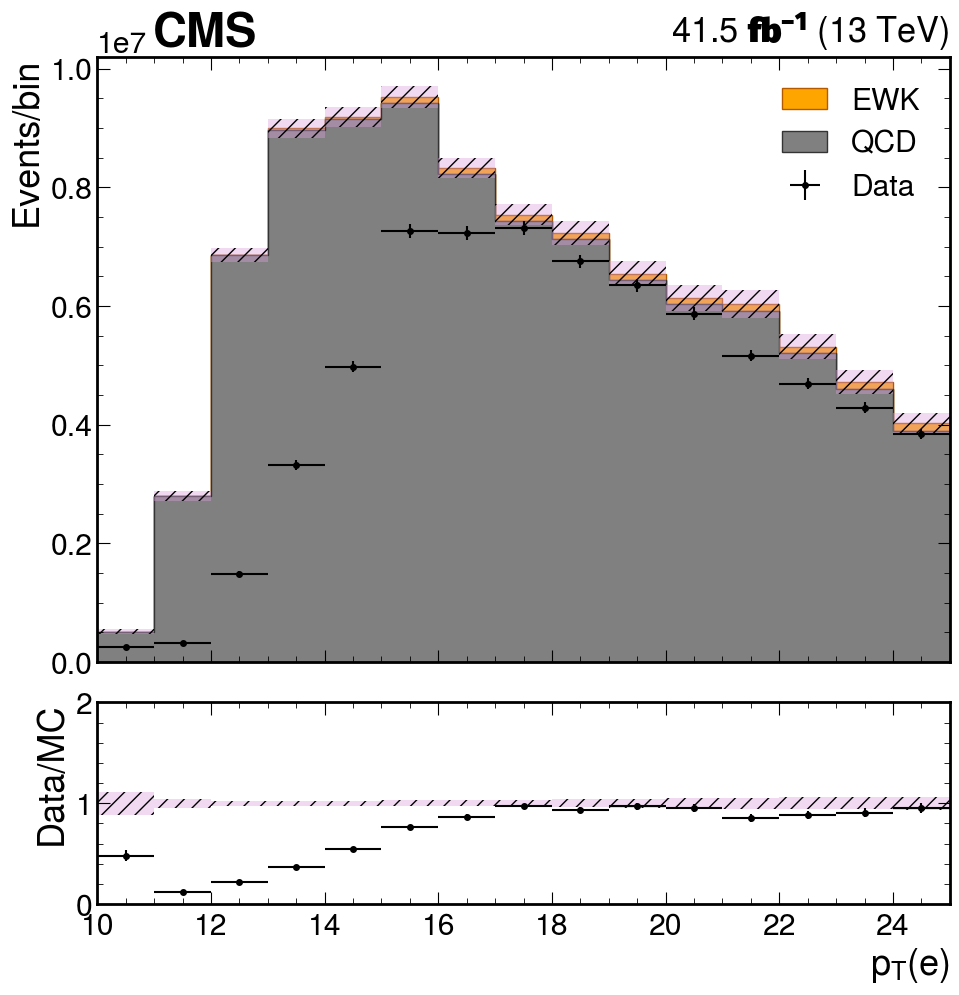
\includegraphics[width=0.45\textwidth]{images/fake_rate/trigger_eff/rawpt_low_Electron_2017.png} \hfill
%   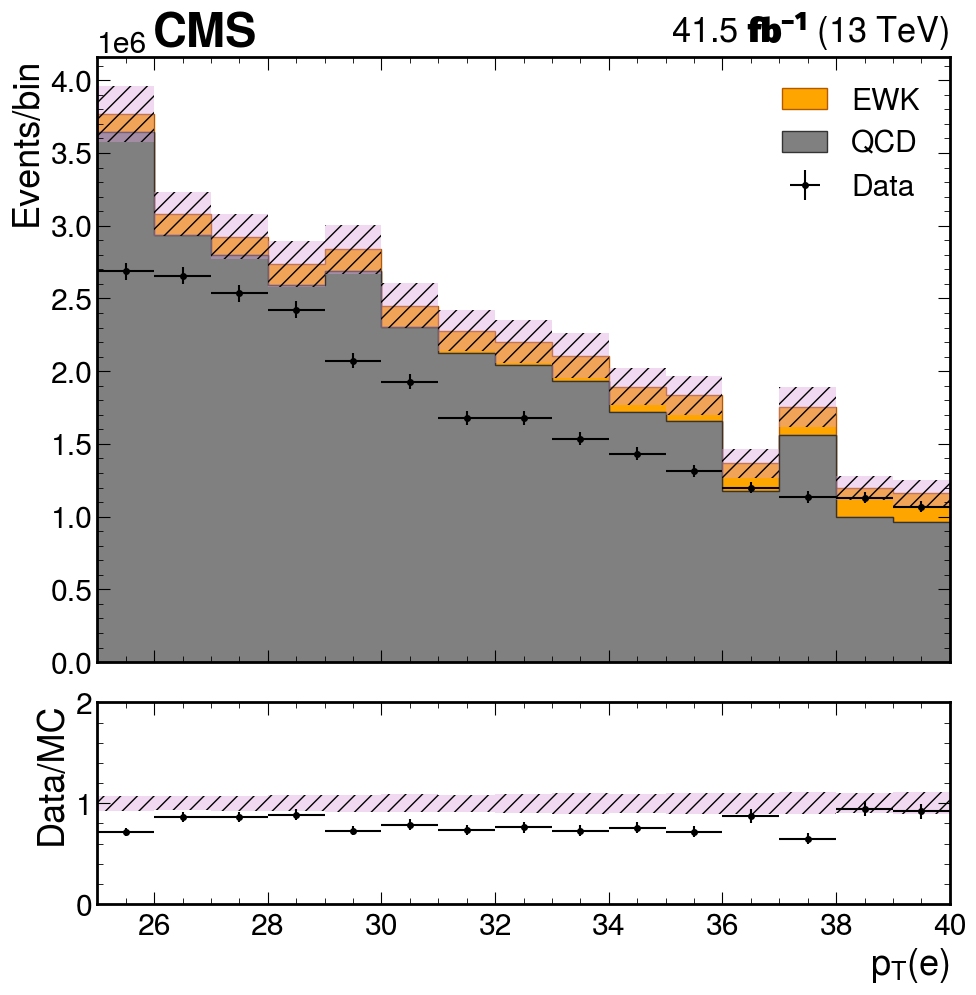
\includegraphics[width=0.45\textwidth]{images/fake_rate/trigger_eff/rawpt_high_Electron_2017.png}\\
%   \caption{Trigger turn-on curves for 2017. Left shows low-pt trigger, right show high-pt trigger. Top shows muons, Bottom Electrons.}\label{fig:2017_trigger_turnon}
% \end{figure}

% \begin{figure}
%   \centering
%   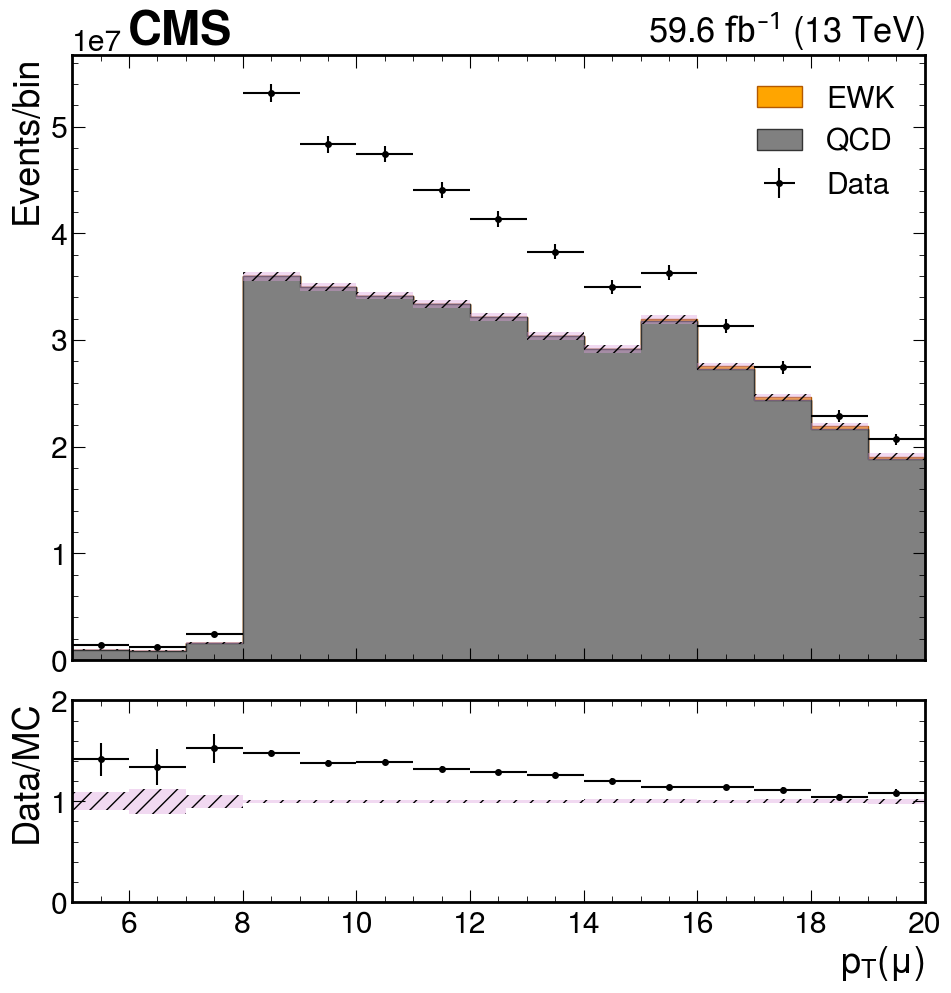
\includegraphics[width=0.45\textwidth]{images/fake_rate/trigger_eff/rawpt_low_Muon_2018.png} \hfill
%   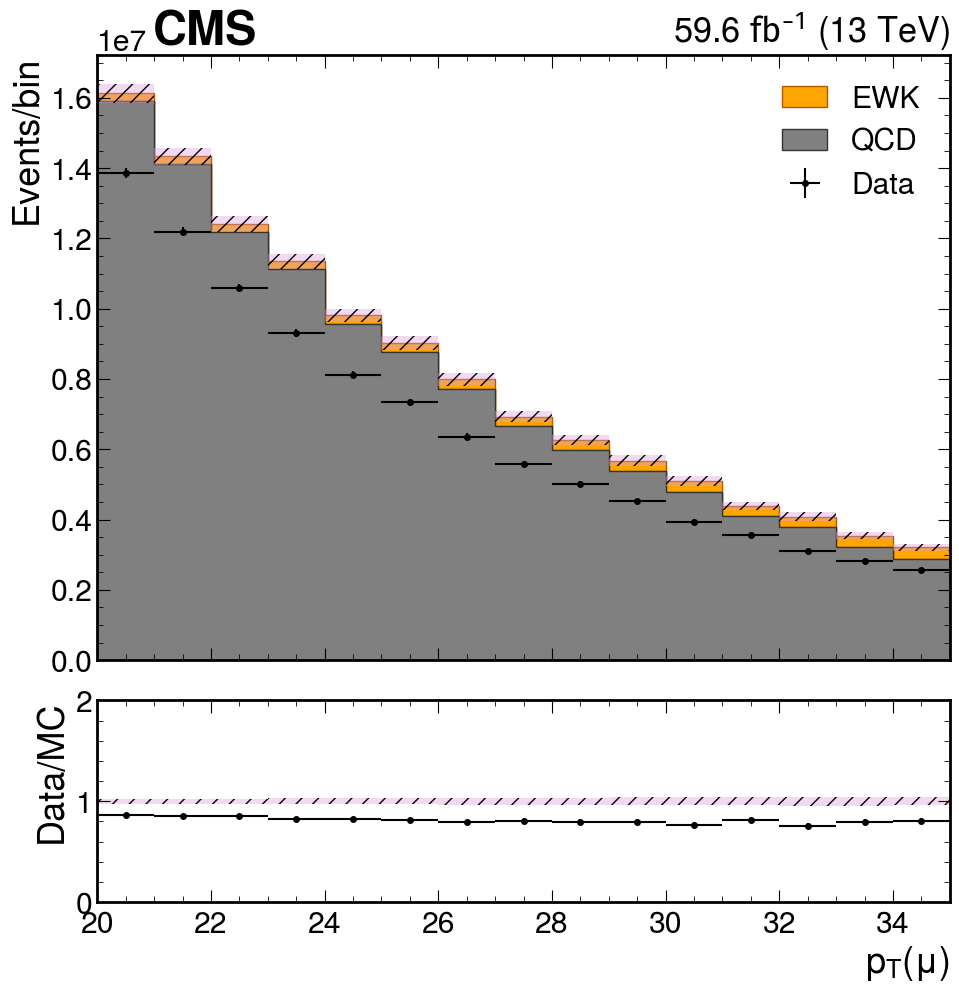
\includegraphics[width=0.45\textwidth]{images/fake_rate/trigger_eff/rawpt_high_Muon_2018.png}\\
%   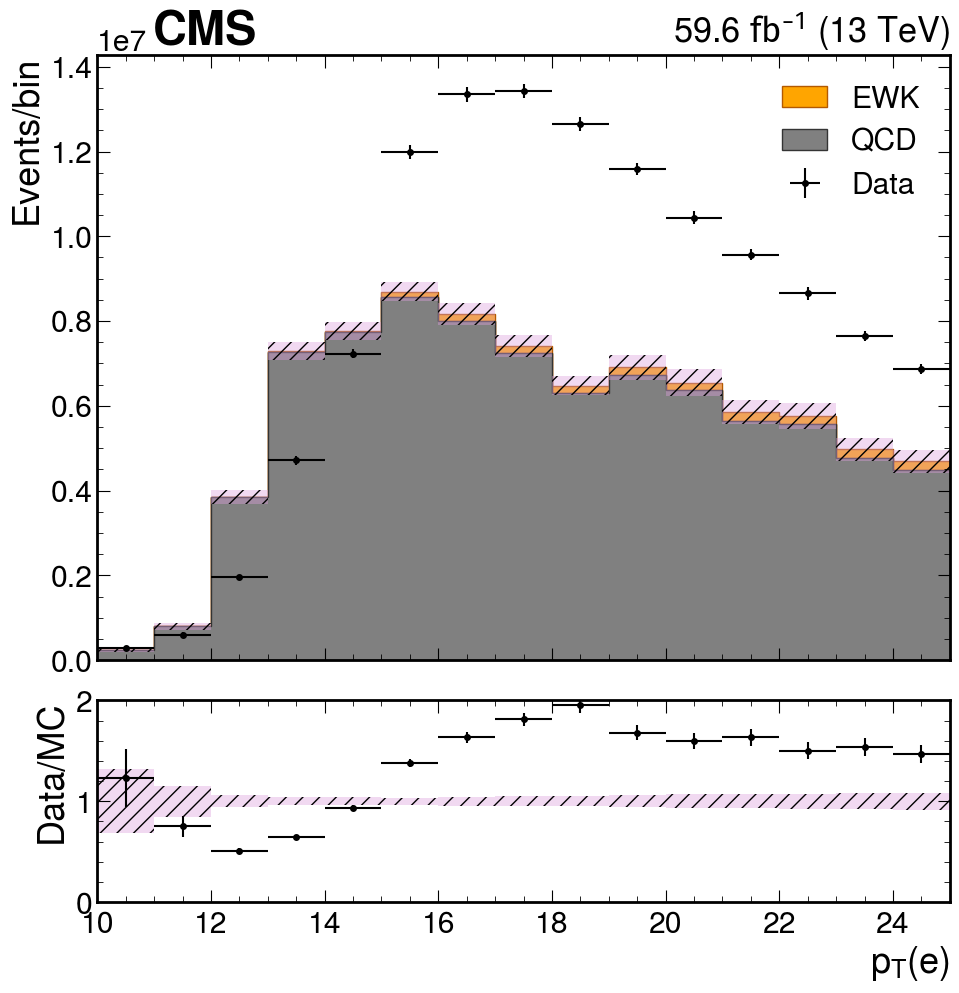
\includegraphics[width=0.45\textwidth]{images/fake_rate/trigger_eff/rawpt_low_Electron_2018.png} \hfill
%   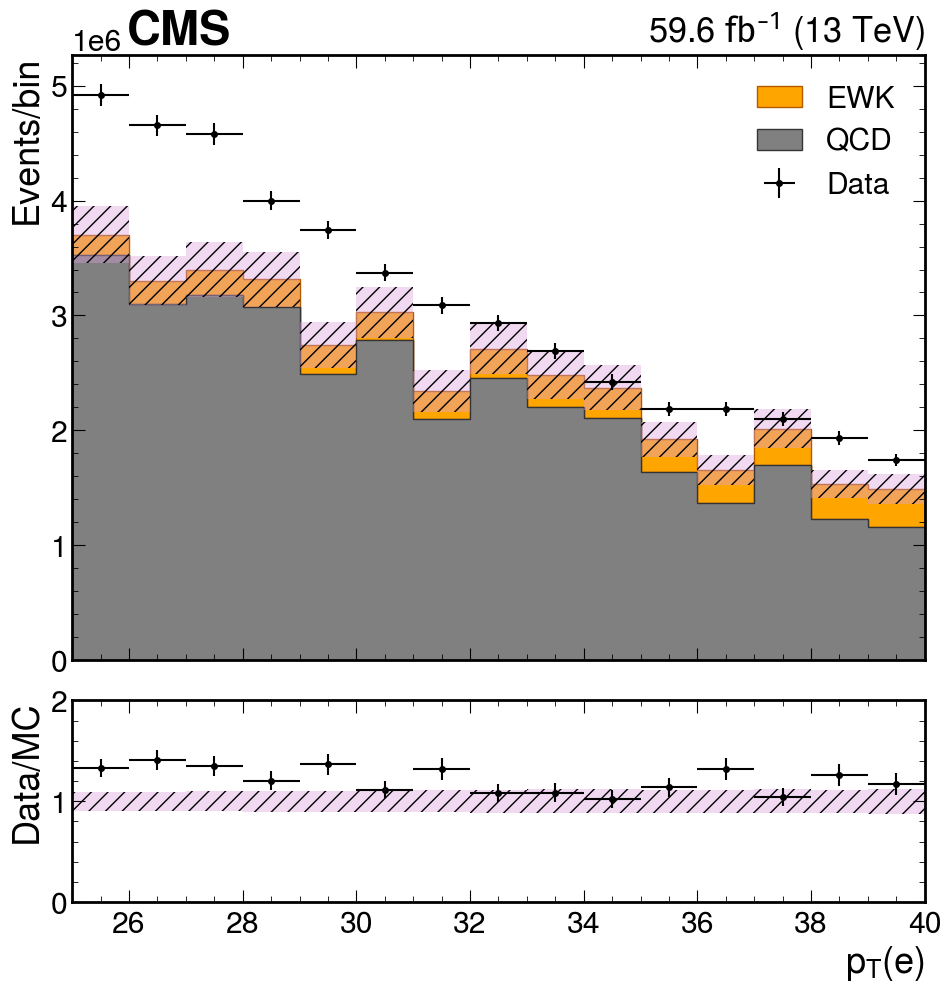
\includegraphics[width=0.45\textwidth]{images/fake_rate/trigger_eff/rawpt_high_Electron_2018.png}\\
%   \caption{Trigger turn-on curves for 2018. Left shows low-pt trigger, right show high-pt trigger. Top shows muons, Bottom Electrons.}\label{fig:2018_trigger_turnon}
% \end{figure}

% These plots are made in our Measurement region (definition in ref............). The Data/MC agreement may not be good because there is no trigger scale factors applied or any rescaling of MC samples, but we can see a general trend in the ratio plot. From this, we see that for the high-pt triggers, the thresholds mentioned before are sufficient enough to have the triggers in the plateau. For the low-pt triggers, we see that we need to cut our Fake Leptons to have a $\pt > 12\gev$ for Muon and $\pt > 15\gev$ for Electrons. This meets a compromise of being in the plateau while also satisfying our baseline $\pt$ requirement of 15 GeV. These cuts are reflected in~\ref{tab:lepton_selection}.

\subsubsection{Momentum Correction}\label{sec:nonprompt:pt_correction}
It has been noted in numerous previous analyses that the agreement for the fake rate increases when using a modified $\pt$ for the Fake defined leptons. Typically this method is done by defining the new Fake Lepton $\pt$ as proportional to the closest-jet's $\pt$. This is becuase it reduces the flavor dependency in the fake rate. For different flavors, the transfer factor differs biasing the fake rate in certain $\pt$ ranges to nonprompt leptons coming from a particular flavor. By using the mother jet's $\pt$, the transfer factor is removed and thus makes our fake rate have better agreement across the $\pt$ spectrum.

The mother jet's $\pt$ is larger than the lepton's $\pt$ and would mean all Fake leptons have a larger $\pt$ than the Tight defined leptons, so we rescale this jet $\pt$ to match the Tight's $\pt$. This gives us our corrected Fake $\pt$ as follows
\begin{equation*}
  \pt \rightarrow f\frac{\pt}{p_{T}^{ratio}}
\end{equation*}
Where $p_{T}^{ratio}$ is the ratio of the lepton's $\pt$ to the mother jet's $\pt$ and f is the factor to rescale our Fake $\pt$ to match our Tight $\pt$.

To calculate this factor f, we look at the average $\pt$ for different TTH mva values (which defines Fake vs Tight Leptons) using the jet $\pt$ for Fake Leptons and ``raw'' $\pt$ for Tight Leptons.

\begin{figure}
  \centering
  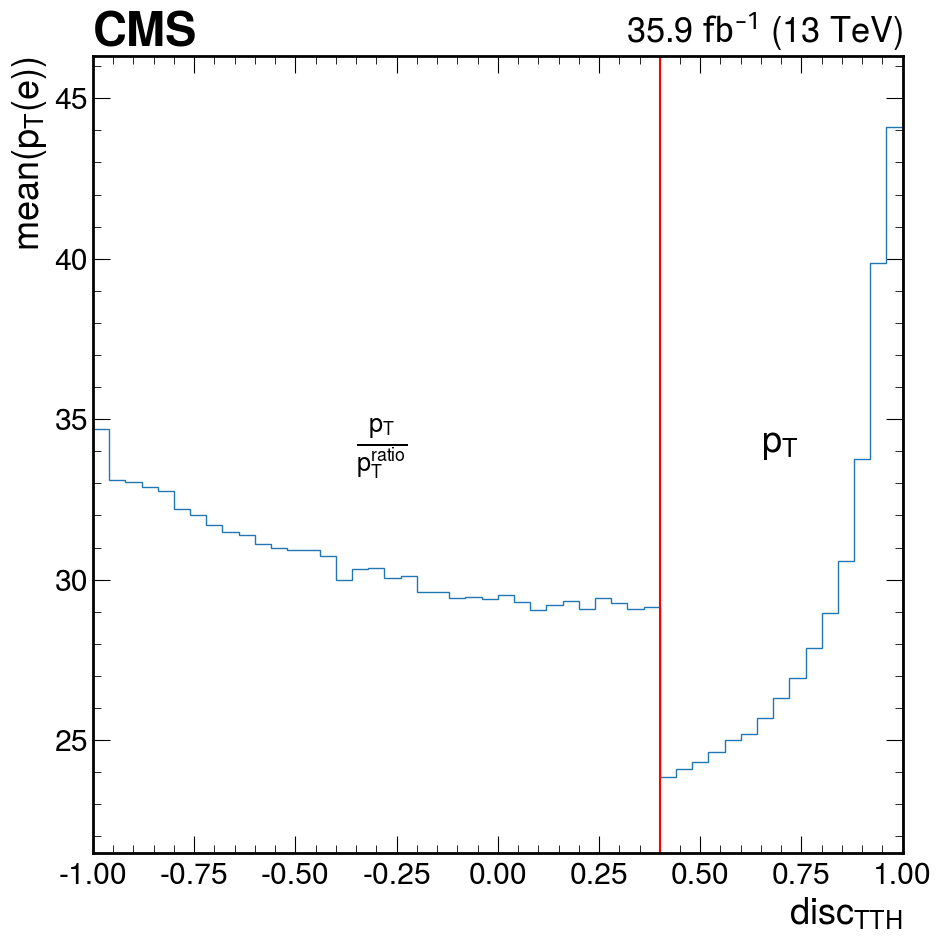
\includegraphics[width=0.45\textwidth]{cone_correction/uncorrected_Electron_0p4_2016.png} \hfill
  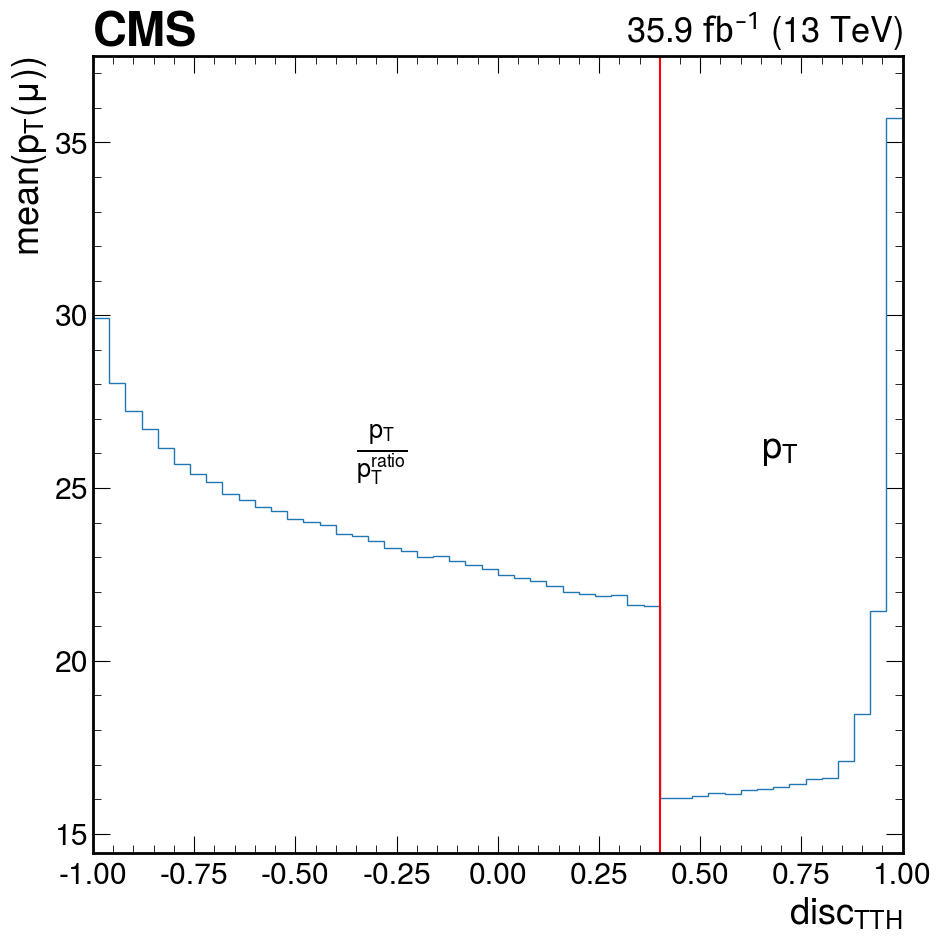
\includegraphics[width=0.45\textwidth]{cone_correction/uncorrected_Muon_0p4_2016.png} \\
  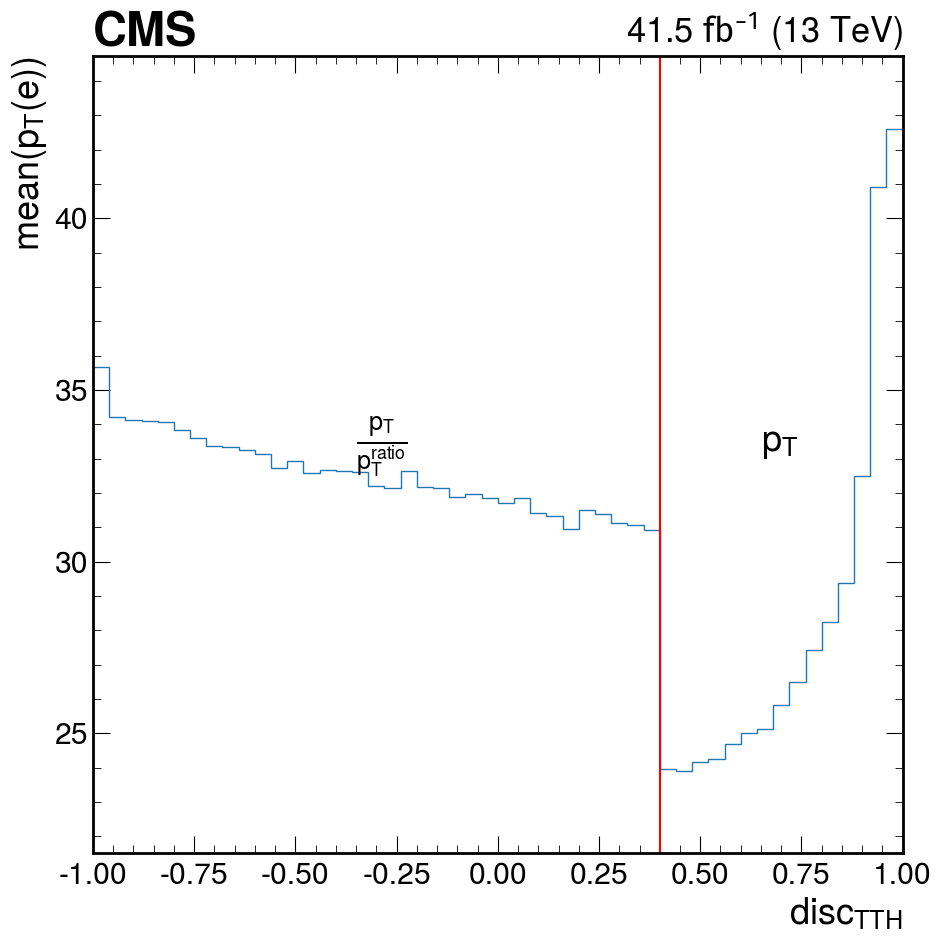
\includegraphics[width=0.45\textwidth]{cone_correction/uncorrected_Electron_0p4_2017.png} \hfill
  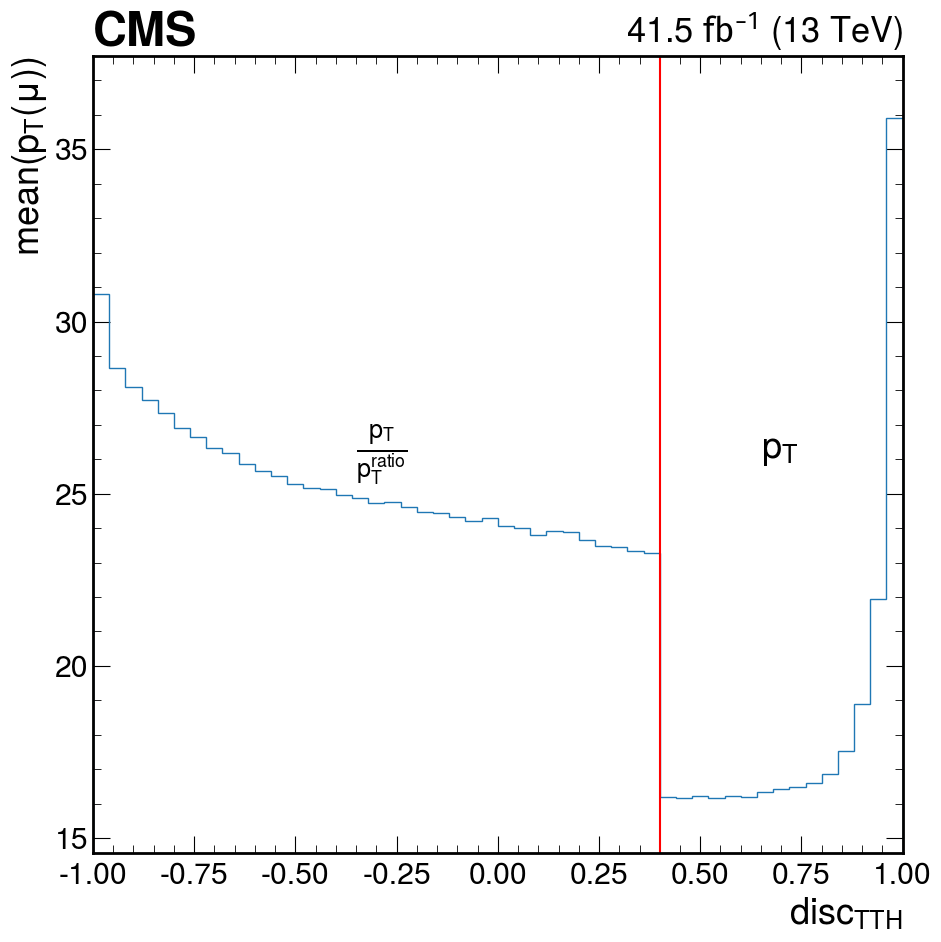
\includegraphics[width=0.45\textwidth]{cone_correction/uncorrected_Muon_0p4_2017.png} \\
  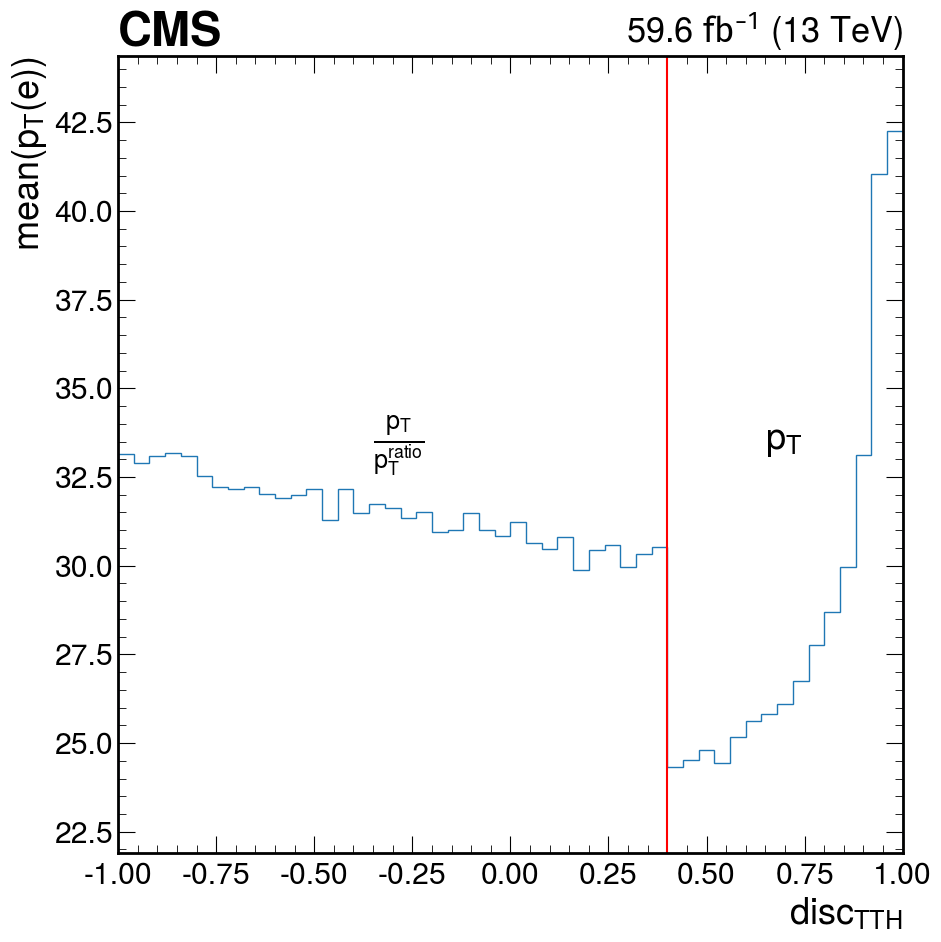
\includegraphics[width=0.45\textwidth]{cone_correction/uncorrected_Electron_0p4_2018.png} \hfill
  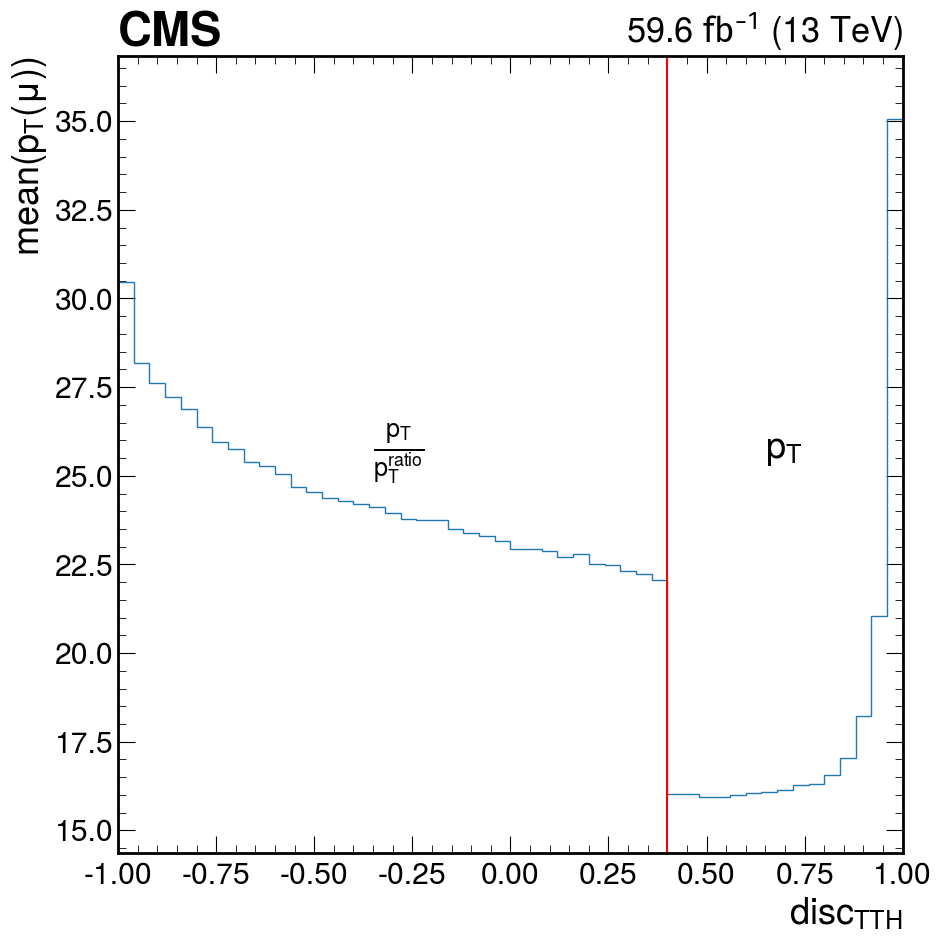
\includegraphics[width=0.45\textwidth]{cone_correction/uncorrected_Muon_0p4_2018.png} \\
  \caption{Average $\pt$ across the TTH mva spectrum for unscaled Fake Leptons. Electrons on the left, Muons on the right, with 2016, 2017, and 2018 respectively for each row}\label{fig:uncorrected_pt}
\end{figure}

\begin{figure}
  \centering
  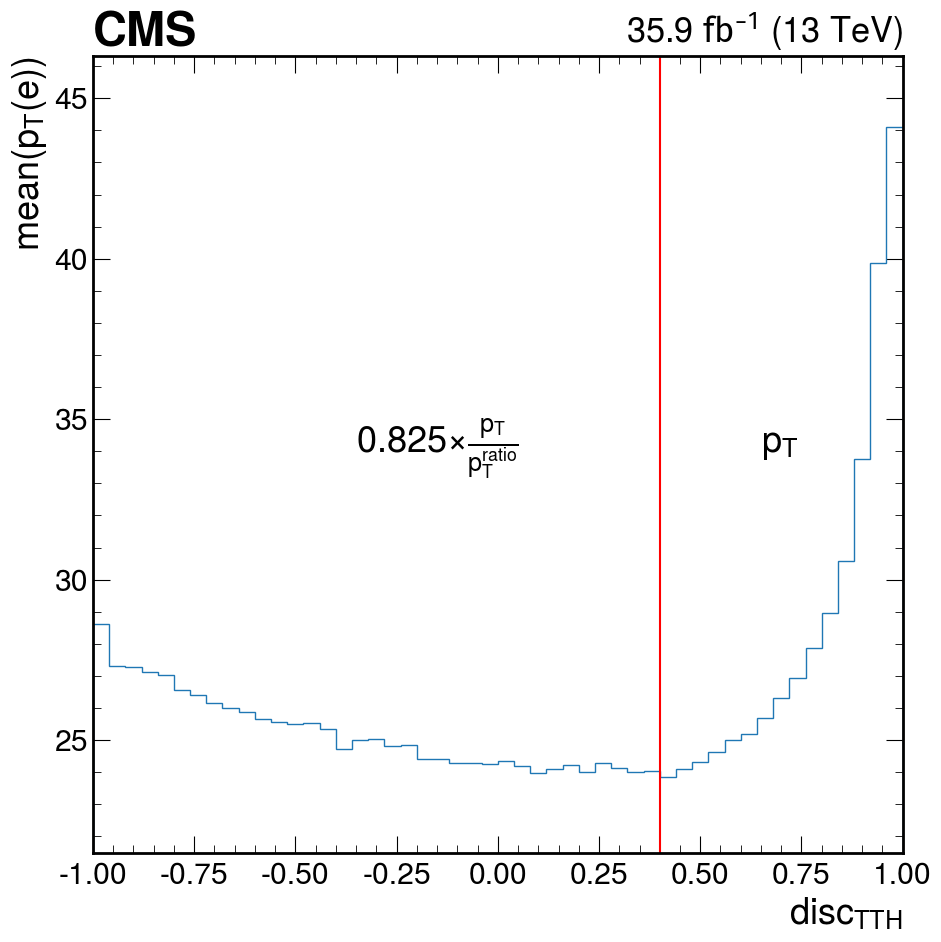
\includegraphics[width=0.45\textwidth]{cone_correction/corrected_Electron_0p4_2016.png} \hfill
  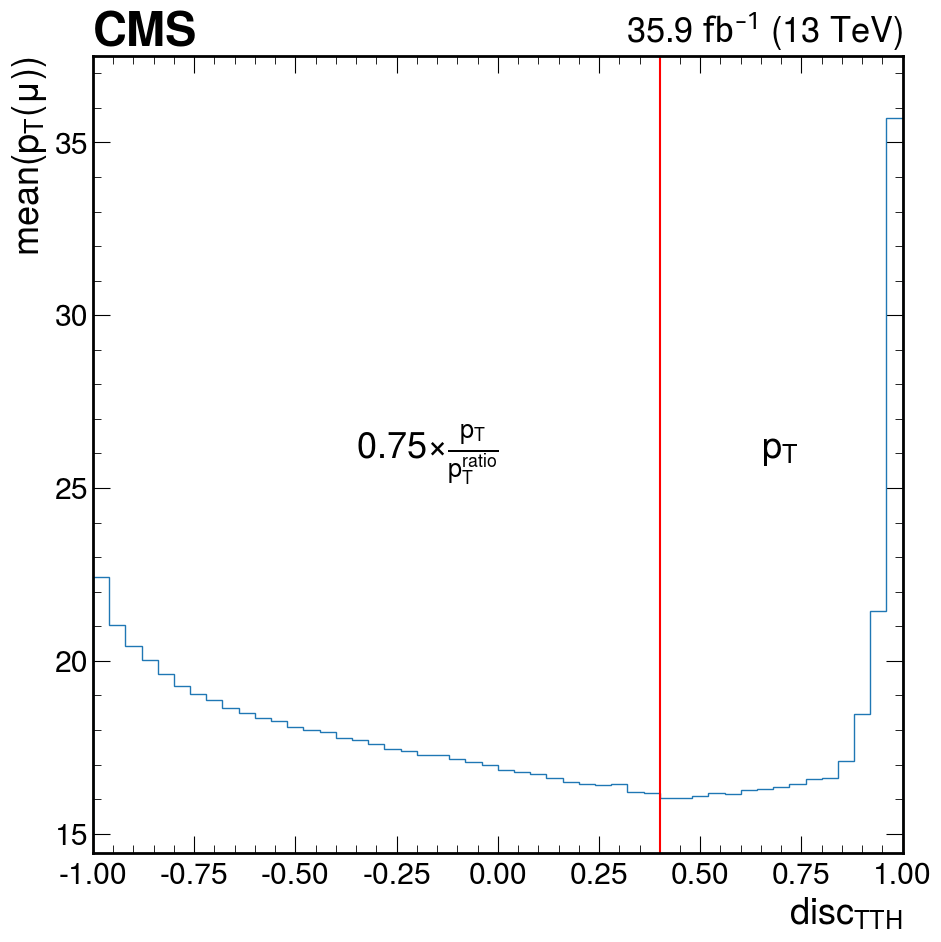
\includegraphics[width=0.45\textwidth]{cone_correction/corrected_Muon_0p4_2016.png} \\
  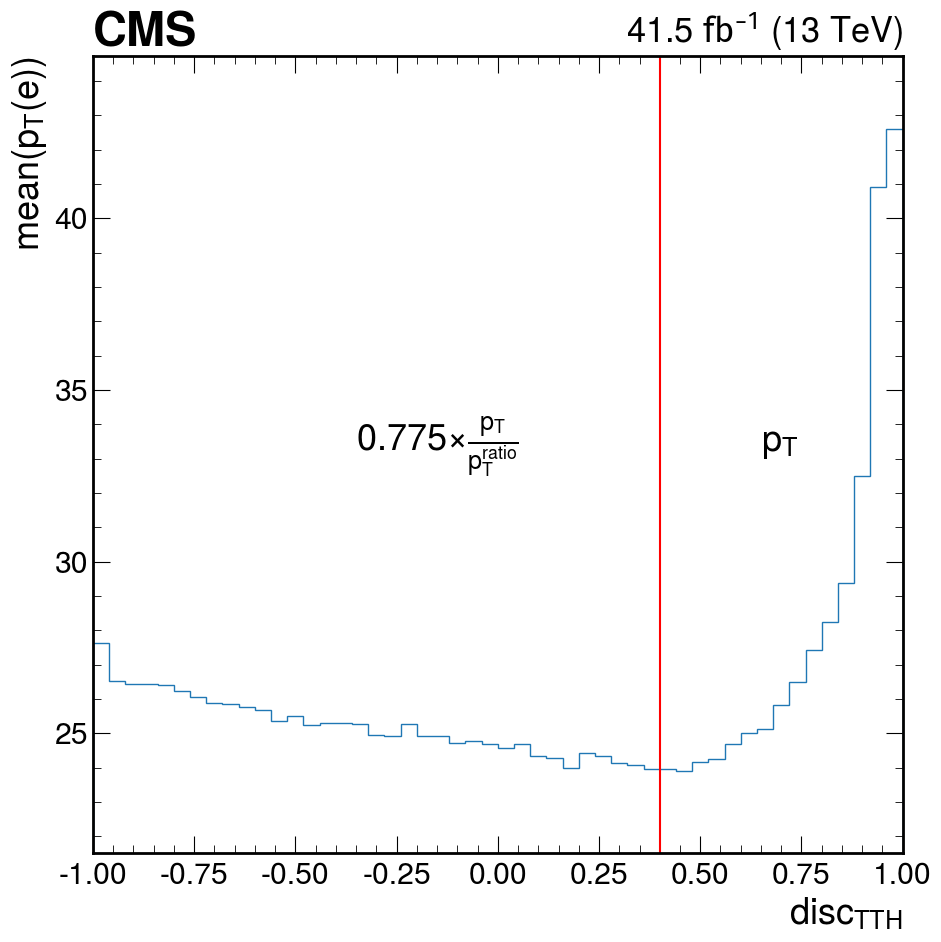
\includegraphics[width=0.45\textwidth]{cone_correction/corrected_Electron_0p4_2017.png} \hfill
  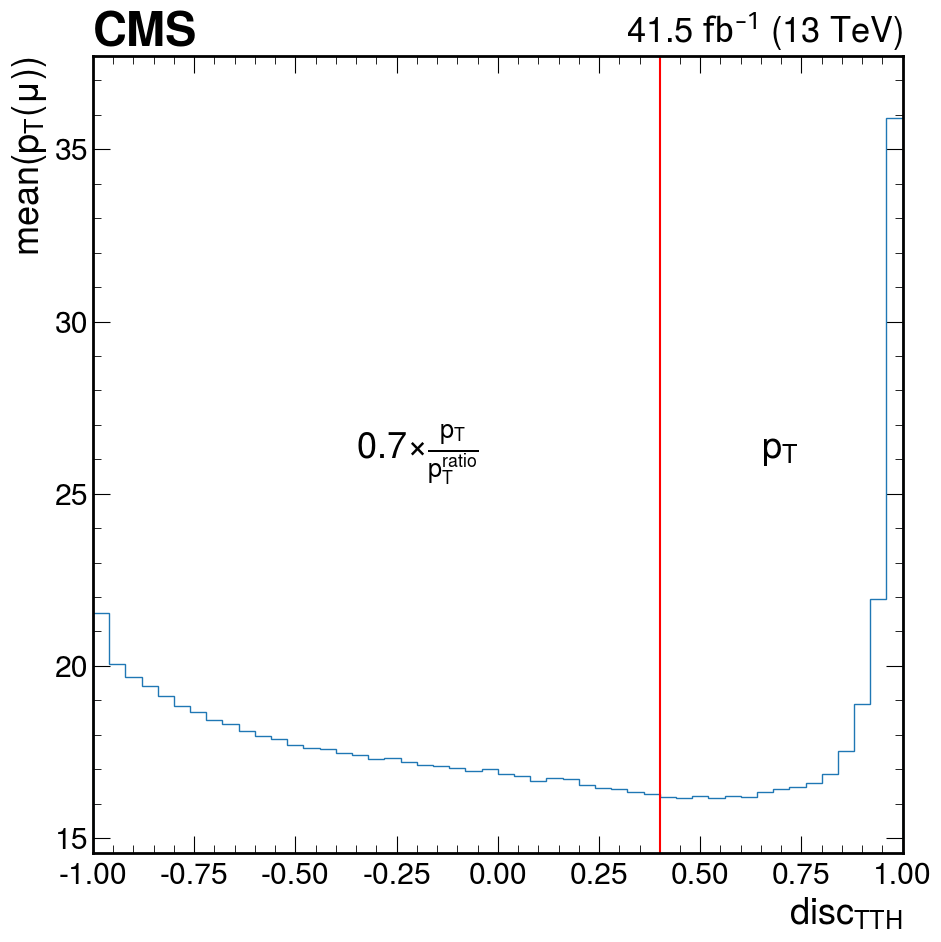
\includegraphics[width=0.45\textwidth]{cone_correction/corrected_Muon_0p4_2017.png} \\
  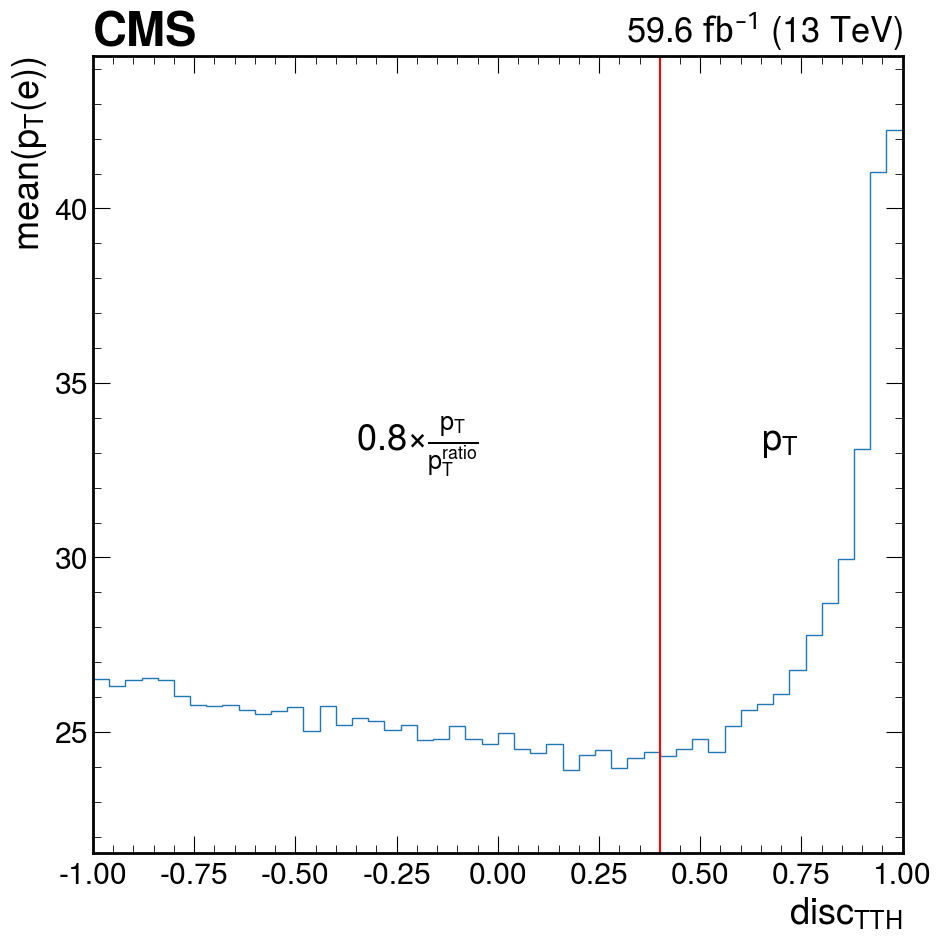
\includegraphics[width=0.45\textwidth]{cone_correction/corrected_Electron_0p4_2018.png} \hfill
  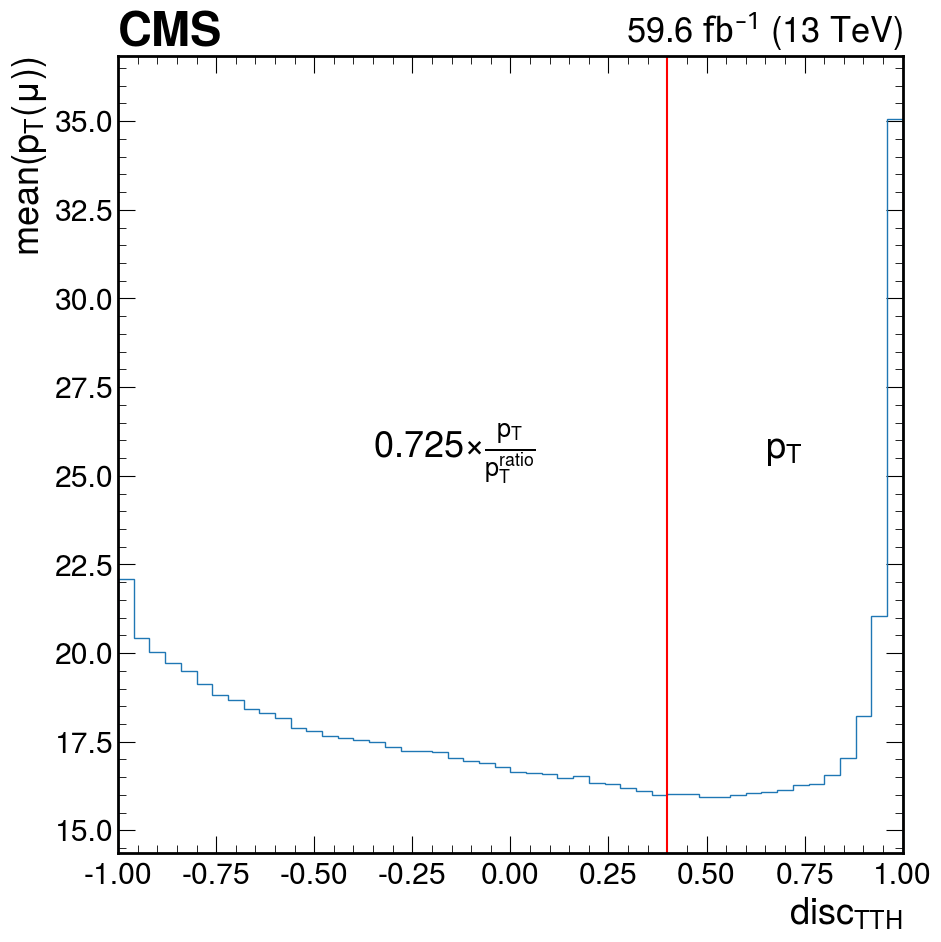
\includegraphics[width=0.45\textwidth]{cone_correction/corrected_Muon_0p4_2018.png} \\
  \caption{Average $\pt$ across the TTH mva spectrum for rescaled Fake Leptons. Electrons on the left, Muons on the right, with 2016, 2017, and 2018 respectively for each row}\label{fig:corrected_pt}
\end{figure}

It should be noted that in defining our leptons, the Fake Lepton is defined with an additional cut on the $p_{T}^{ratio}$. This reduces the number of soft leptons and the overall skewing of the $\pt$ of leptons (\ie{} low $\pt$ leptons that have their momentum scaled up significantly by a large $\pt$ mother jet). While the $p_{T}^{ratio}$ has little effect on the overall fake rate, it has a larger role is setting the $\pt$-correction factor, so a moderate cut is applied to remove most soft Fake Leptons while also not reduce the statistics significantly.

\subsubsection{Jet Flavor Breakdown}\label{sec:nonprompt:flavor_breakdown}
As stated before, our signal region is composed mainly of nonprompt background coming from ttbar because we apply cuts to enrich the number of tops for higher signal efficiency. This means that a higher percentage of nonprompt leptons will be originating from B-jets rather than from lighter flavors. This can be problematic in our fake rate measurement because our QCD multijet measurement region may have a different flavor composition giving a different fake rate. To combat this, we require a recoiling jet to pass one of the btagging Working Points as specified by the BTagging POG.\@ To decide which WP to use, we can look at the MC and see what percentage of leptons come from different flavor jets for our measurement region and closure region and choose the WP that aligns the measurement region closest to the closure region:

\begin{table}
  \centering
  \caption{Tables showing the origin of the lepton for Electron (left) and Muons (right). The percentages are calculated in the measurement regions for the 3 btagging WPs for the recoiing jet as well as no btagging requirement. The last line of the group shows the percentages found in the closure region. The row bolded simply shows the WP with the best agreement to closure}\label{tab:lepton_nonprompt_percentages}
  \begin{tabular}{c c c c c }
    \hline
    year                  & Btag WP & \% B   & \% C   & \% light \\
    \hline
    \multirow{5}{*}{2016} & None    & 55.7\% & 12.3\%  & 7.5\%    \\
                          & Loose   & 73.0\% & 9.0\%  & 3.4\%    \\
                          & Medium  & 85.4\% & 5.1\%  & 1.8\%    \\
                          & Tight   & 90.6\% & 2.3\%  & 1.4\%    \\
                          & Closure & 76.6\% & 1.1\%  & 3.8\%    \\
    \hline
    \multirow{5}{*}{2017} & None    & 55.5\% & 12.1\% & 6.8\%    \\
                          & Loose   & 70.6\% & 9.4\%  & 3.9\%    \\
                          & Medium  & 83.8\% & 4.9\%  & 2.8\%    \\
                          & Tight   & 91.1\% & 1.7\%  & 2.0\%    \\
                          & Closure & 78.8\% & 1.4\%  & 3.2\%    \\
    \hline
    \multirow{5}{*}{2018} & None    & 56.3\% & 11.9\%  & 6.3\%    \\
                          & Loose   & 68.9\% & 9.3\%  & 4.9\%    \\
                          & Medium  & 85.2\% & 4.6\%  & 2.4\%    \\
                          & Tight   & 90.7\% & 1.9\%  & 2.3\%    \\
                          & Closure & 76.2\% & 1.3\%  & 3.7\%    \\
    \hline
  \end{tabular}
  \qquad
  \begin{tabular}{c c c c c}
    \hline
    year                  & Btag WP & \% B   & \% C   & \%light \\
    \hline
    \multirow{5}{*}{2016} & None    & 70.0\% & 20.7\% & 5.7\%   \\
                          & Loose   & 81.1\% & 13.5\% & 2.9\%   \\
                          & Medium  & 89.7\% & 7.0\% & 1.7\%      \\
                          & Tight   & 94.1\% & 3.3\% & 1.3\%      \\
                          & Closure & 94.2\% & 2.6\%  & 0.8\%   \\
    \hline
    \multirow{5}{*}{2017} & None    & 68.0\% & 21.4\% & 6.5\%   \\
                          & Loose   & 77.9\% & 15.6\% & 3.4\%   \\
                          & Medium  & 88.1\% & 7.1\%  & 1.6\%   \\
                          & Tight   & 92.5\% & 3.5\%  & 1.2\%   \\
                          & Closure & 93.7\% & 2.5\%  & 0.7\%   \\
    \hline
    \multirow{5}{*}{2018} & None    & 68.6\% & 21.1\% & 6.4\%   \\
                          & Loose   & 78.3\% & 15.0\% & 3.6\%   \\
                          & Medium  & 89.4\% & 7.0\%  & 1.7\%   \\
                          & Tight   & 94.7\% & 2.8\%  & 1.2\%   \\
                          & Closure & 92.9\% & 3.0\%  & 0.8\%   \\
    \hline
  \end{tabular}
\end{table}
While the best bjet cut across years seems to be Loose for Electrons and Tight for muons, we relax these cuts to allow for more statistics. In the measurement region, we don't apply a cut on the bjet for electrons and require a medium btagged jet for muons. This compromise doesn't seem to affect the fake rate significantly while allowing for higher precision from the gain in statistics.

\subsubsection{Templated Fit}\label{sec:nonprompt:template_fit}
Our fake rate is derived from data by subtracting the prompt contribution from it, in which the prompt comes from MC.\@ The MC that corresponds to the prompt contribution is ttbar, Drell-Yan, W+Jets, or what we call EWK MC.\@ In our QCD multijet region, MC may not model data as accurately and trigger scale factors need to be applied for our 4 heavily prescaled triggers. To improve this agreement, we fit the shapes of the MC to data in a side band region. The Sideband region is defined the same as our measurement region with the MET cut inverted (and the requirement of a tight lepton):

\begin{itemize}
  \item Pass single Lepton trigger (trigger by $\pt$)
  \item 1 Tight Lepton
  \item $N_{j} = 1$ with $\Delta R(j, \ell) > 1$
  \item $\MET > 30\gev$
\end{itemize}

For this templated fit, we split our MC into two groups, EWK (as states before) and QCD.\@ Using the shapes of the QCD and EWK in our $\mT$ distribution, we find the QCD and EWK scale factors that minimize the chi-squared to data. To account for differences in the scaling that depend on $\pt$, the Sideband region is divided into regions based on the $\pt$ binning of the fake rate. This means a template fit is done per $\pt$ bin. By finding a scale factor for EWK and QCD, we also remove the need for applying trigger scale factors since the template fit scales the overall MC normalization to data as would be done with the trigger scale factors.

\begin{figure}
  \centering
  \subfigure(1) 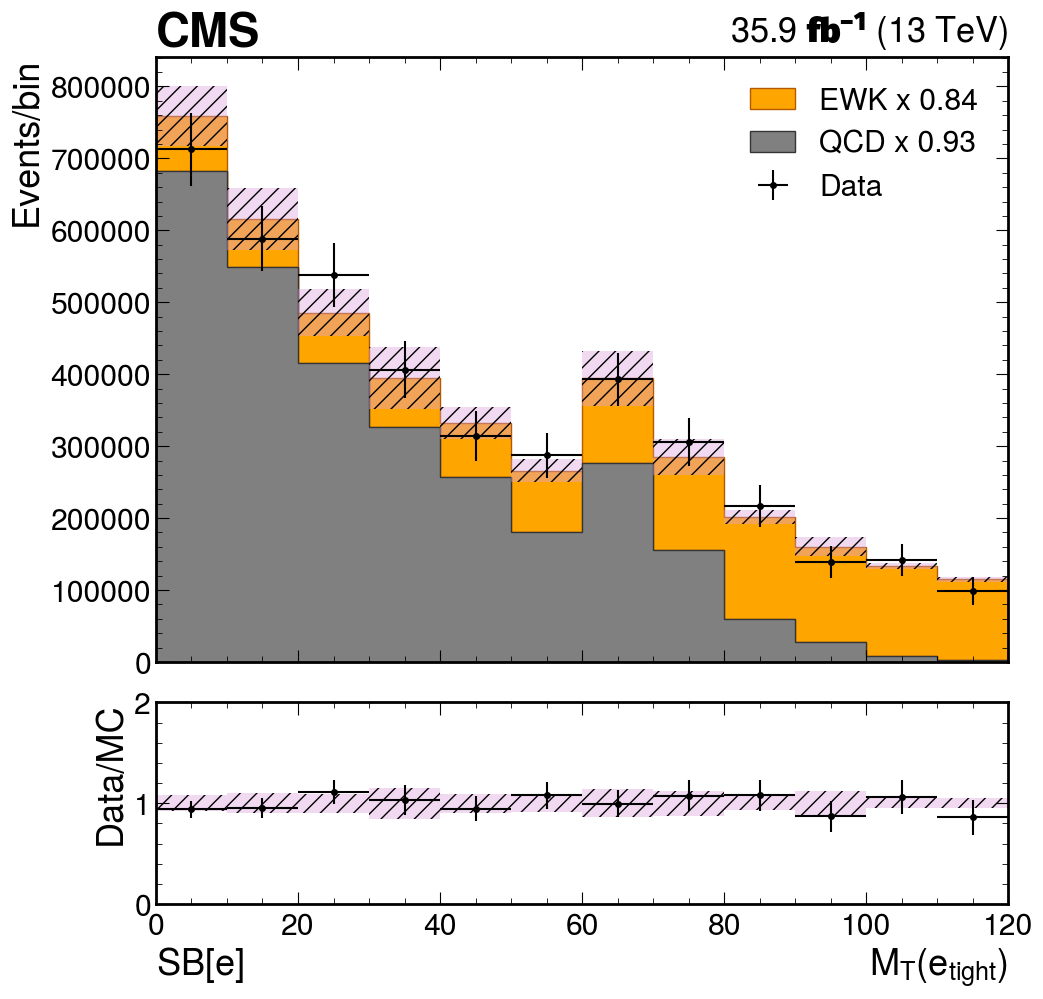
\includegraphics[width=0.35\textwidth]{template_fit/2016/mt_low_Electron_15.0.png} \hfill
  \subfigure(2) 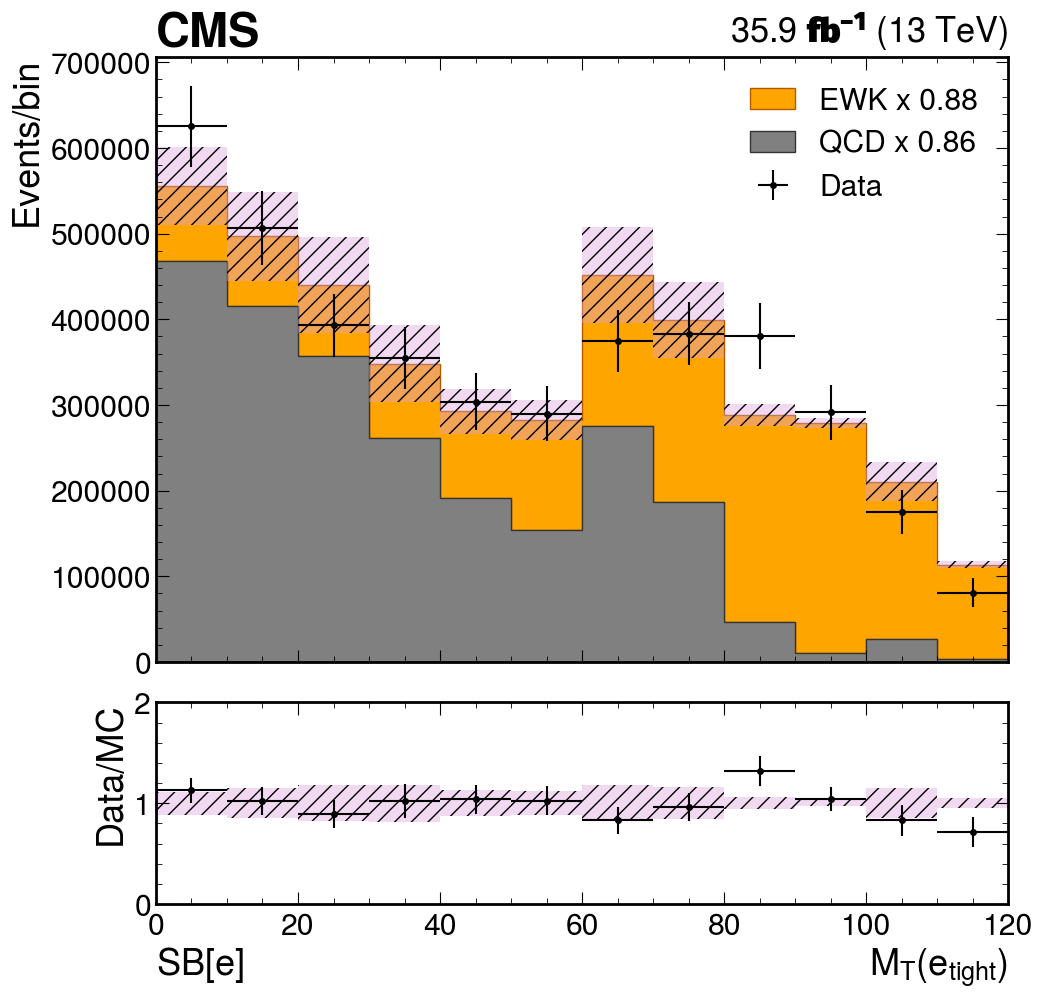
\includegraphics[width=0.35\textwidth]{template_fit/2016/mt_low_Electron_20.0.png} \\
  \subfigure(3) 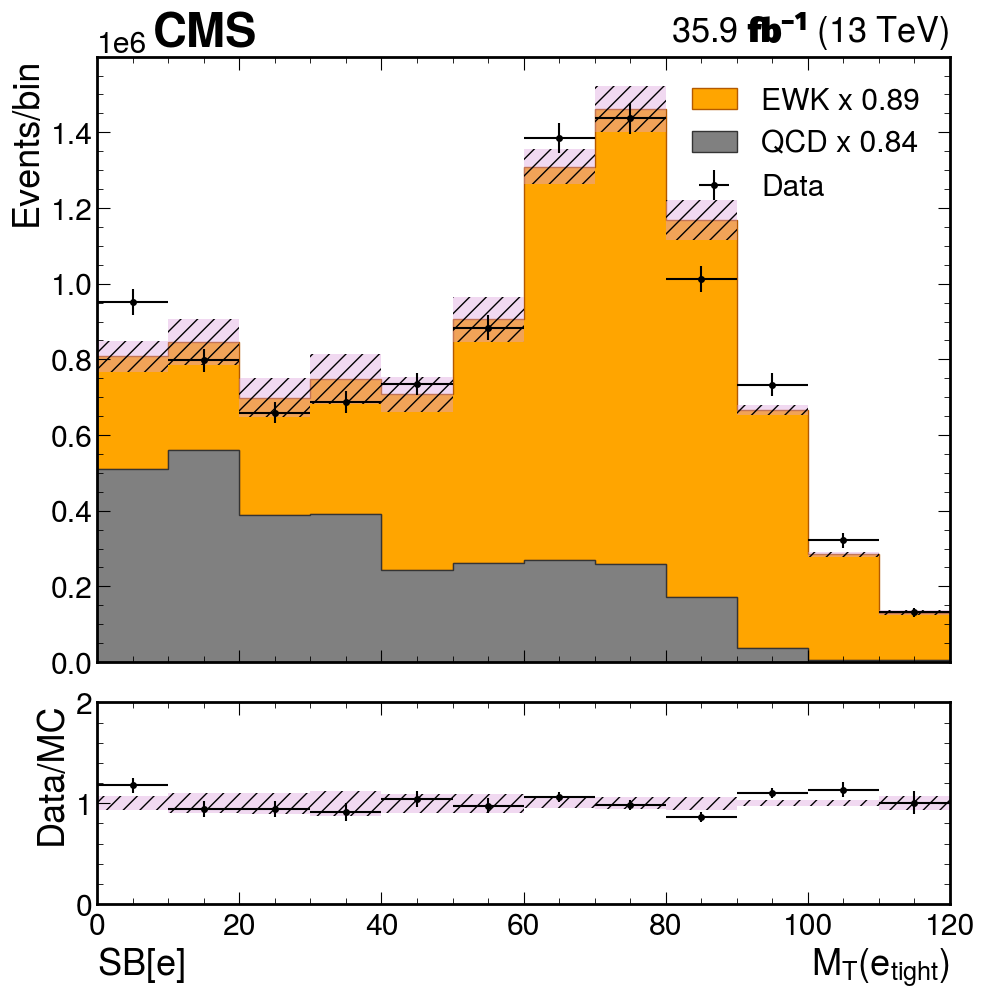
\includegraphics[width=0.35\textwidth]{template_fit/2016/mt_high_Electron_25.0.png} \hfill
  \subfigure(4) 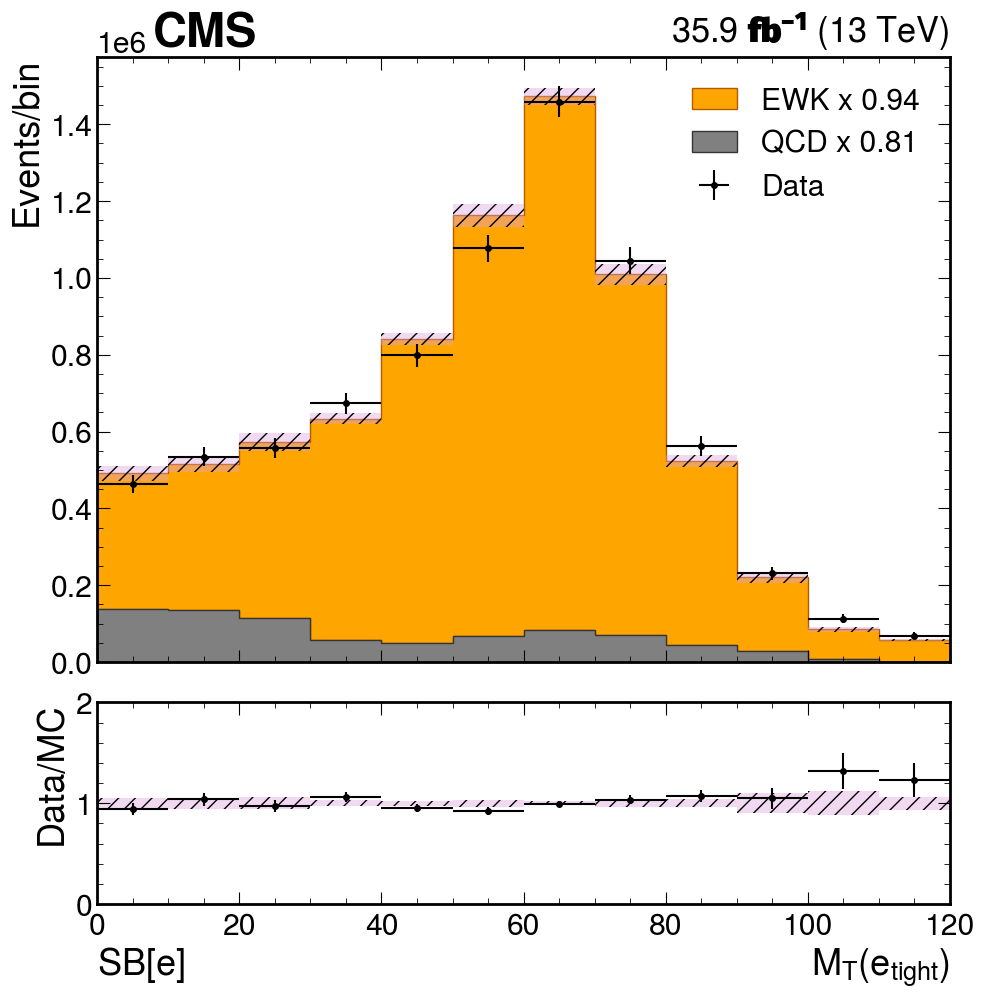
\includegraphics[width=0.35\textwidth]{template_fit/2016/mt_high_Electron_45.0.png} \\
  \subfigure(5) 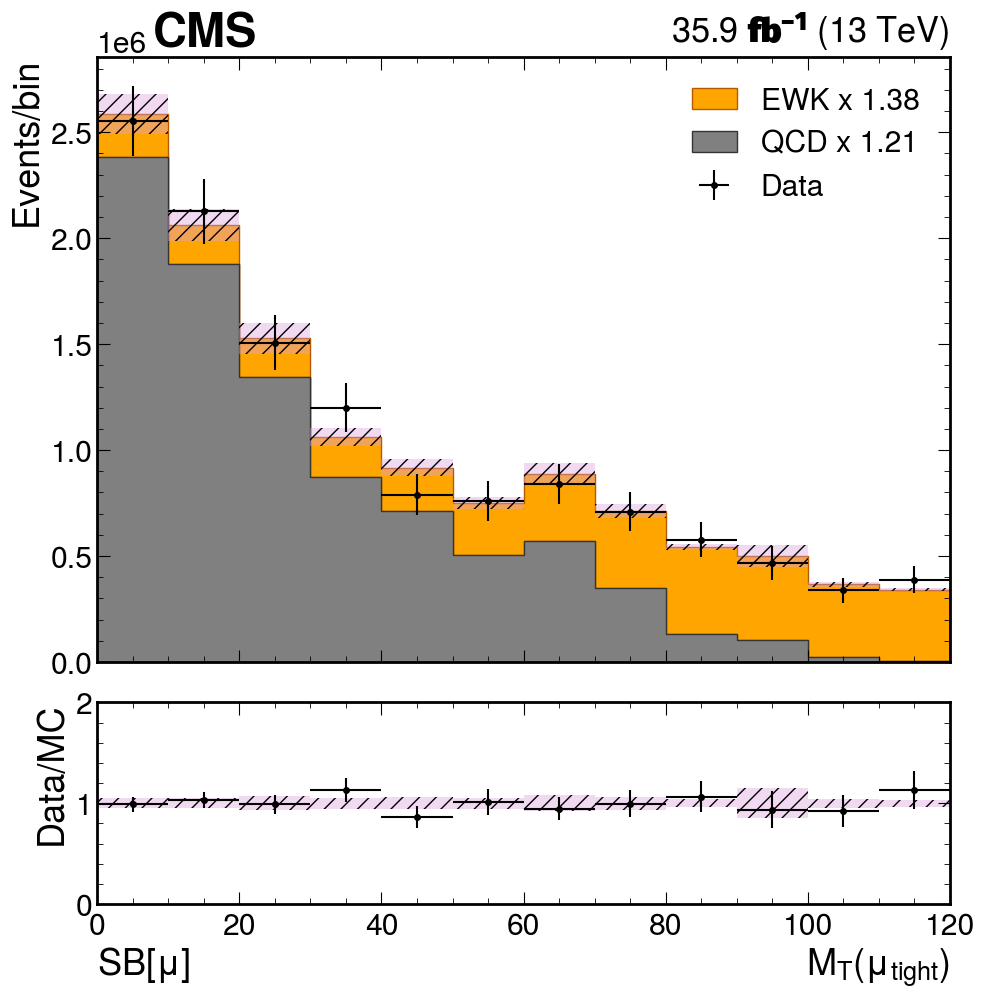
\includegraphics[width=0.35\textwidth]{template_fit/2016/mt_low_Muon_15.0.png} \hfill
  \subfigure(6) 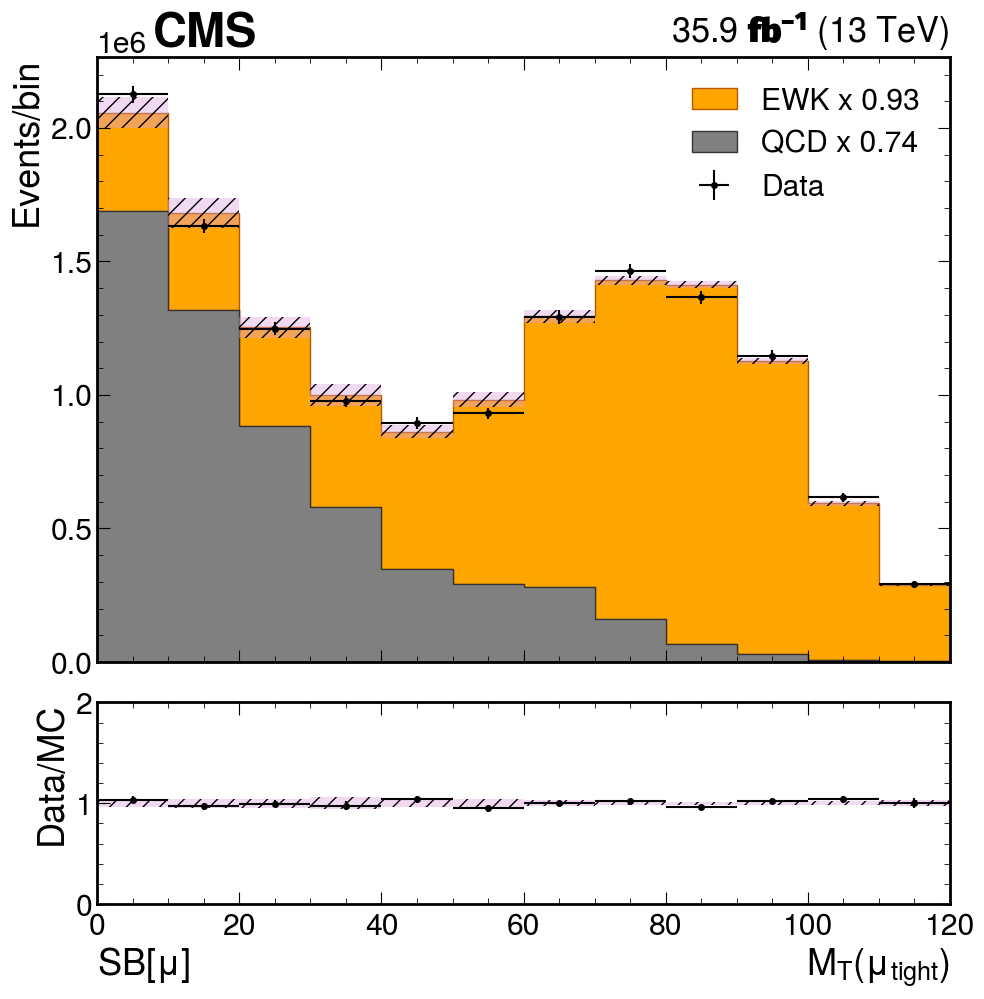
\includegraphics[width=0.35\textwidth]{template_fit/2016/mt_high_Muon_20.0.png} \\
  \subfigure(7) 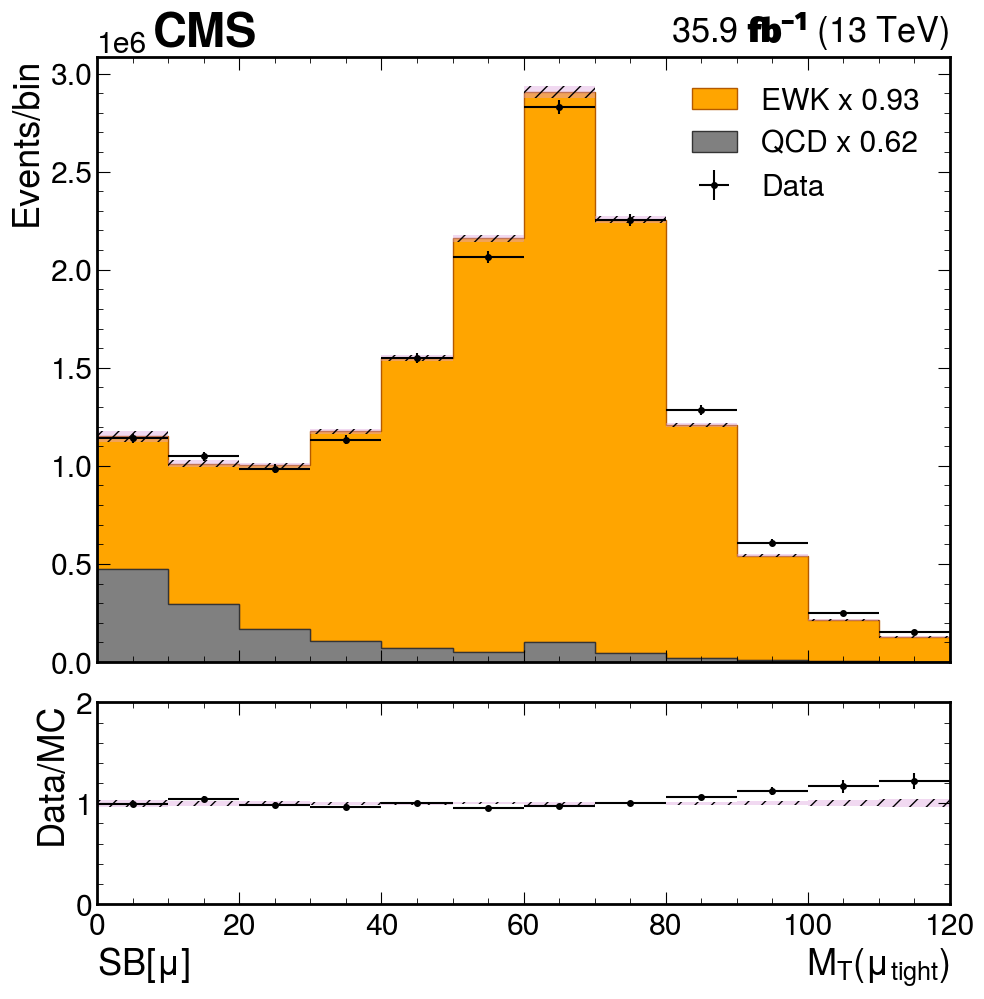
\includegraphics[width=0.35\textwidth]{template_fit/2016/mt_high_Muon_35.0.png}
  \caption{Results of the Template fit for 2016. Top 4 plots are for Electrons for the $\pt$ ranges of $\pt < 20\gev$ (1), $20\gev<\pt<25\gev$ (2), $25\gev<\pt<45\gev$ (3), and $\pt>45\gev$ (4), while the bottom 3 plots are for Muons in the $\pt$ ranges of $\pt < 20\gev$ (5), $20\gev<\pt<35\gev$ (6), and $\pt>35\gev$ (7)}
\end{figure}

\begin{figure}
  \centering
  \subfigure(1) 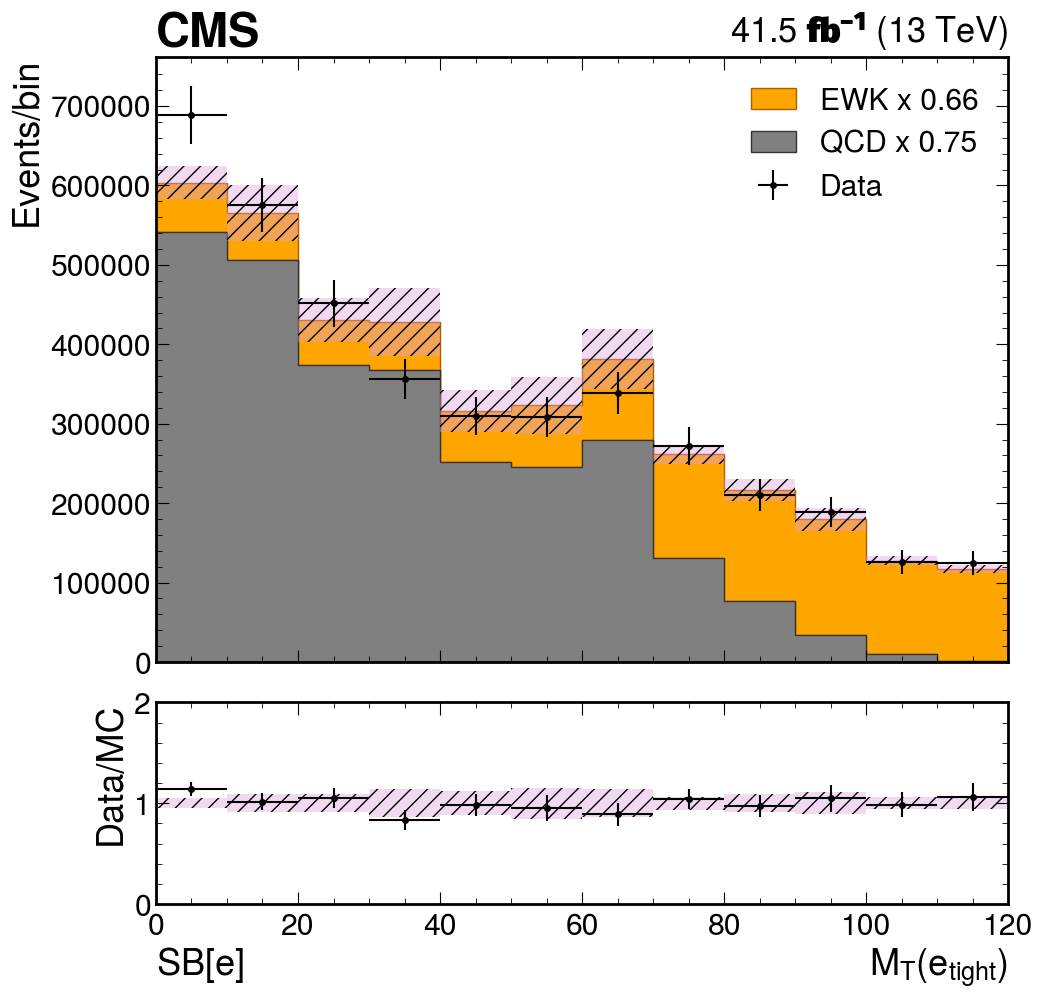
\includegraphics[width=0.35\textwidth]{template_fit/2017/mt_low_Electron_15.0.png} \hfill
  \subfigure(2) 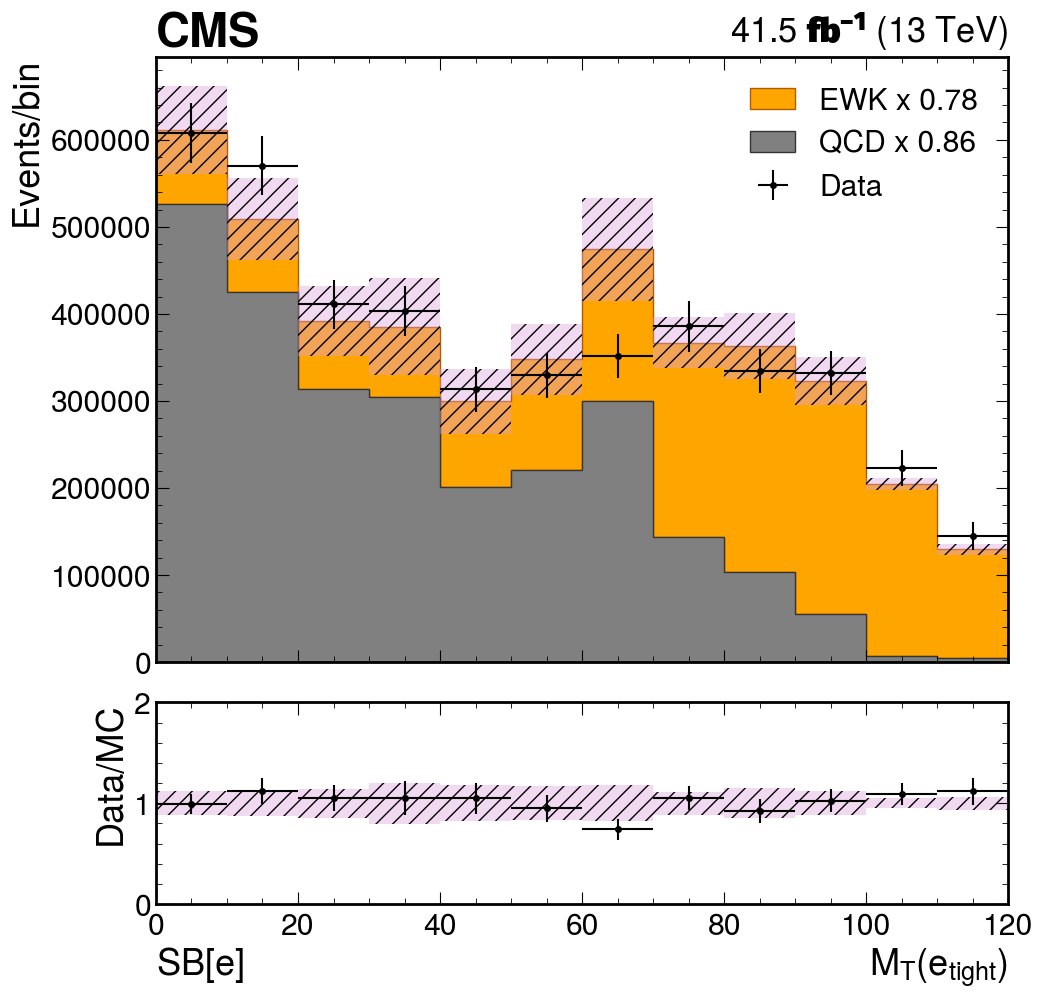
\includegraphics[width=0.35\textwidth]{template_fit/2017/mt_low_Electron_20.0.png} \\
  \subfigure(3) 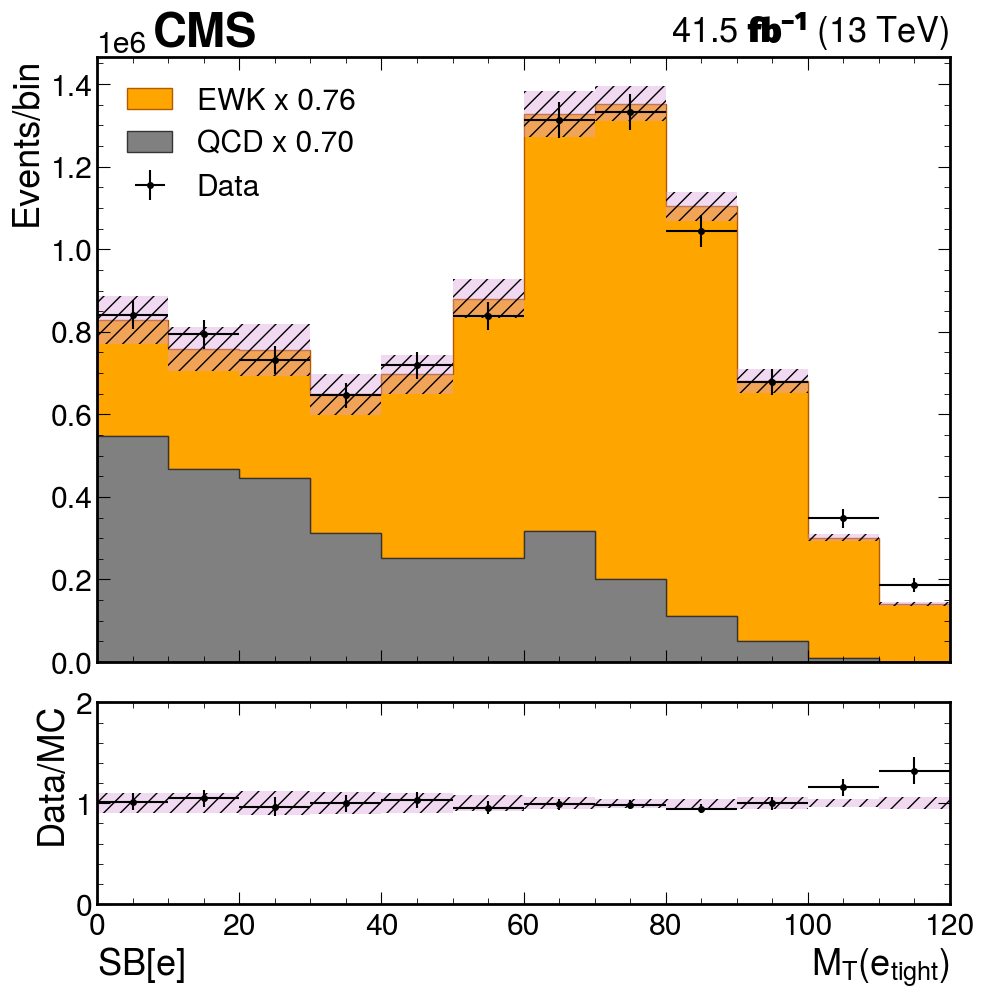
\includegraphics[width=0.35\textwidth]{template_fit/2017/mt_high_Electron_25.0.png} \hfill
  \subfigure(4) 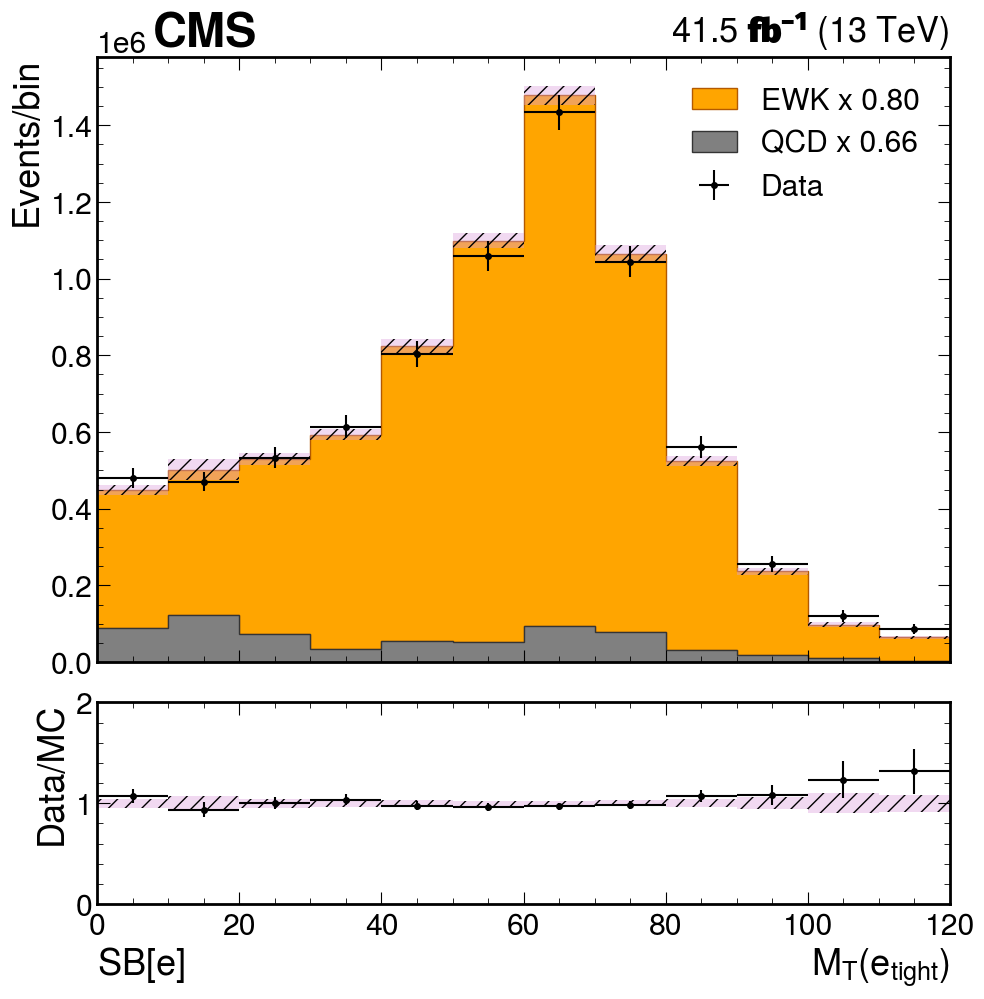
\includegraphics[width=0.35\textwidth]{template_fit/2017/mt_high_Electron_45.0.png} \\
  \subfigure(5) 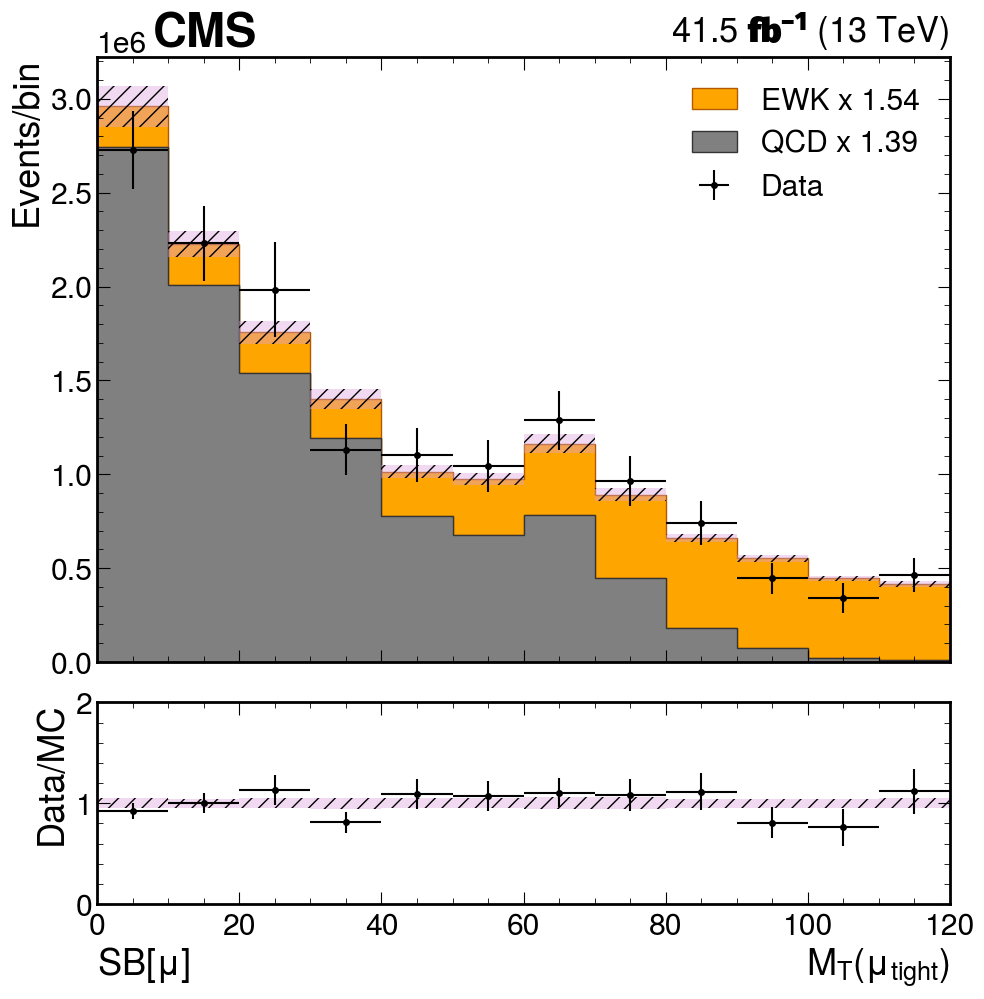
\includegraphics[width=0.35\textwidth]{template_fit/2017/mt_low_Muon_15.0.png} \hfill
  \subfigure(6) 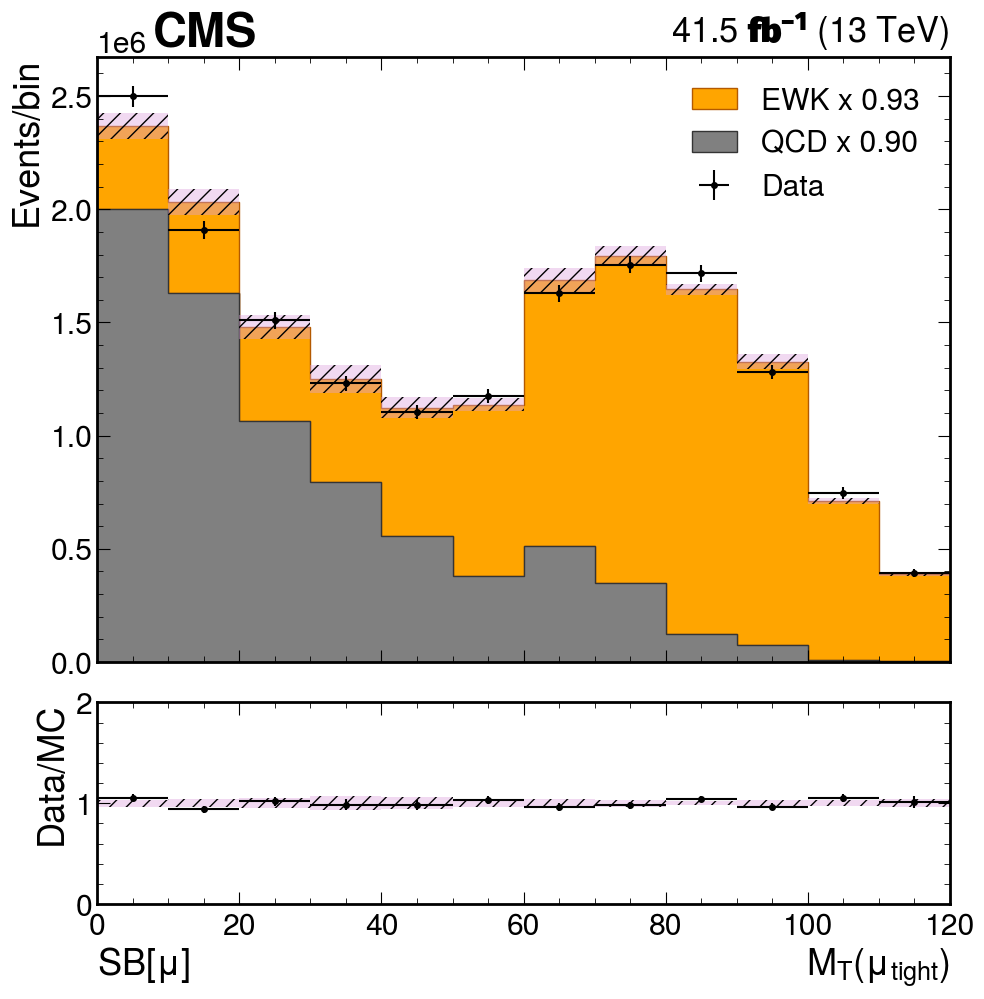
\includegraphics[width=0.35\textwidth]{template_fit/2017/mt_high_Muon_20.0.png} \\
  \subfigure(7) 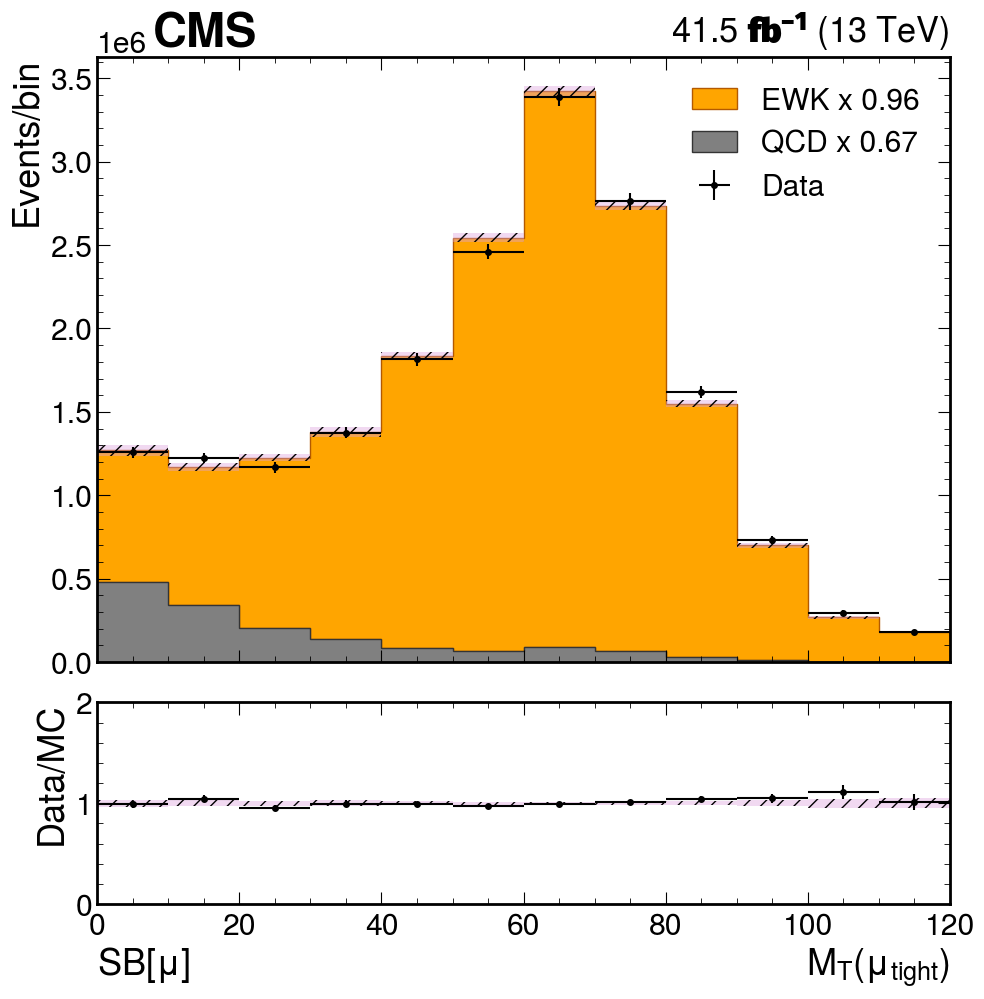
\includegraphics[width=0.35\textwidth]{template_fit/2017/mt_high_Muon_35.0.png}
  \caption{Results of the Template fit for 2017. Top 4 plots are for Electrons for the $\pt$ ranges of $\pt < 20\gev$ (1), $20\gev<\pt<25\gev$ (2), $25\gev<\pt<45\gev$ (3), and $\pt>45\gev$ (4), while the bottom 3 plots are for Muons in the $\pt$ ranges of $\pt < 20\gev$ (5), $20\gev<\pt<35\gev$ (6), and $\pt>35\gev$ (7)}
\end{figure}

\begin{figure}
  \centering
  \subfigure(1) 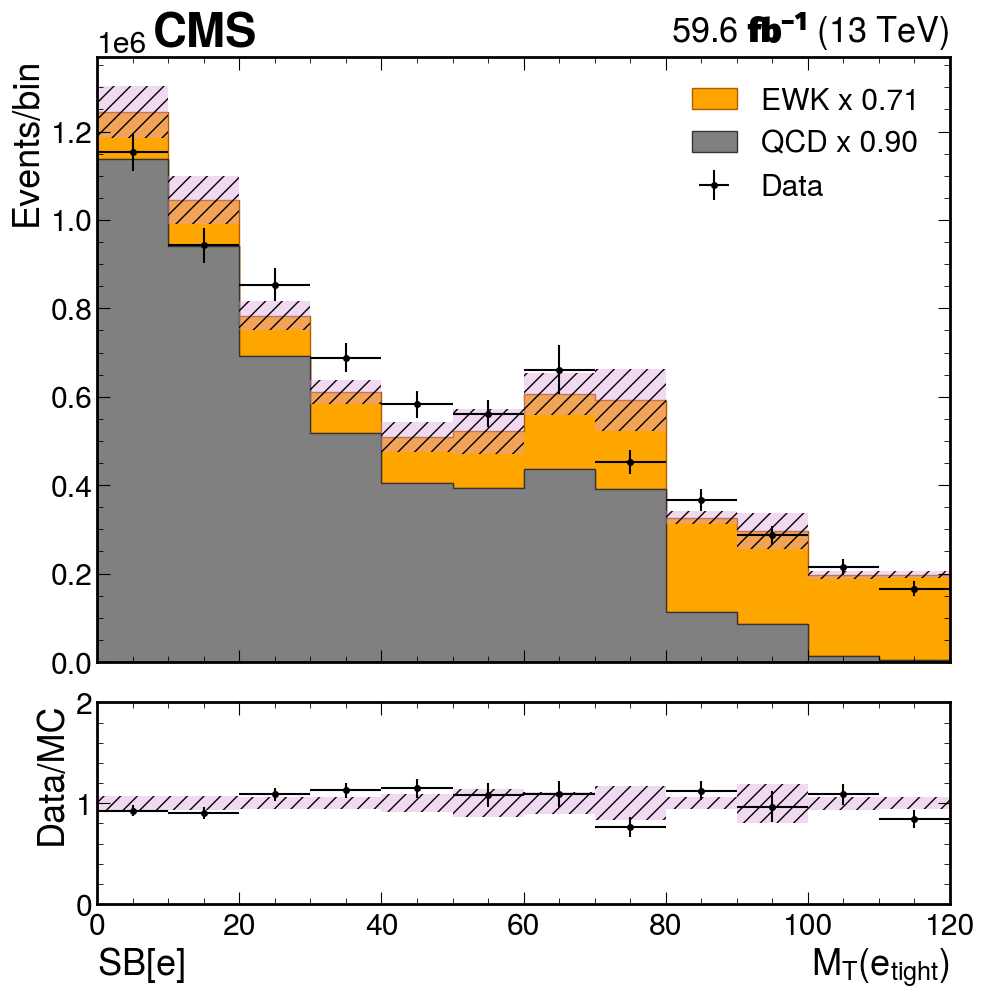
\includegraphics[width=0.35\textwidth]{template_fit/2018/mt_low_Electron_15.0.png} \hfill
  \subfigure(2) 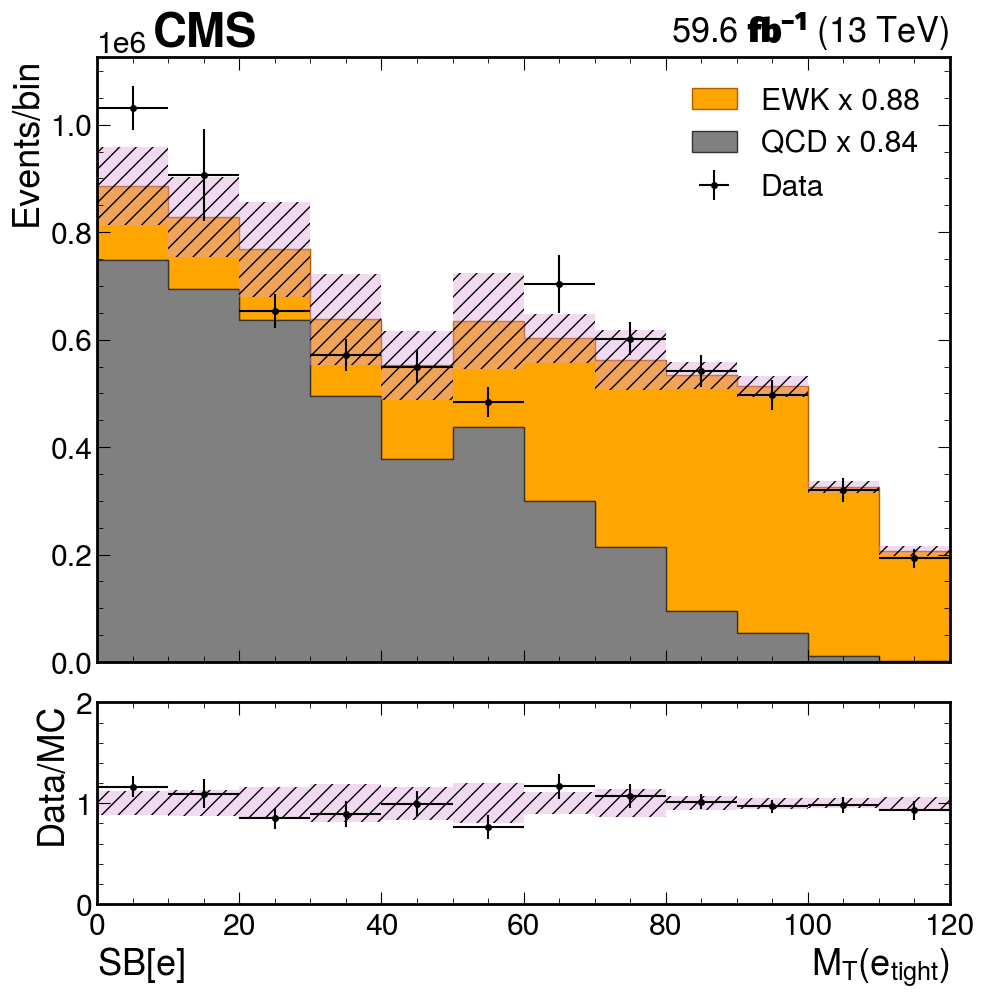
\includegraphics[width=0.35\textwidth]{template_fit/2018/mt_low_Electron_20.0.png} \\
  \subfigure(3) 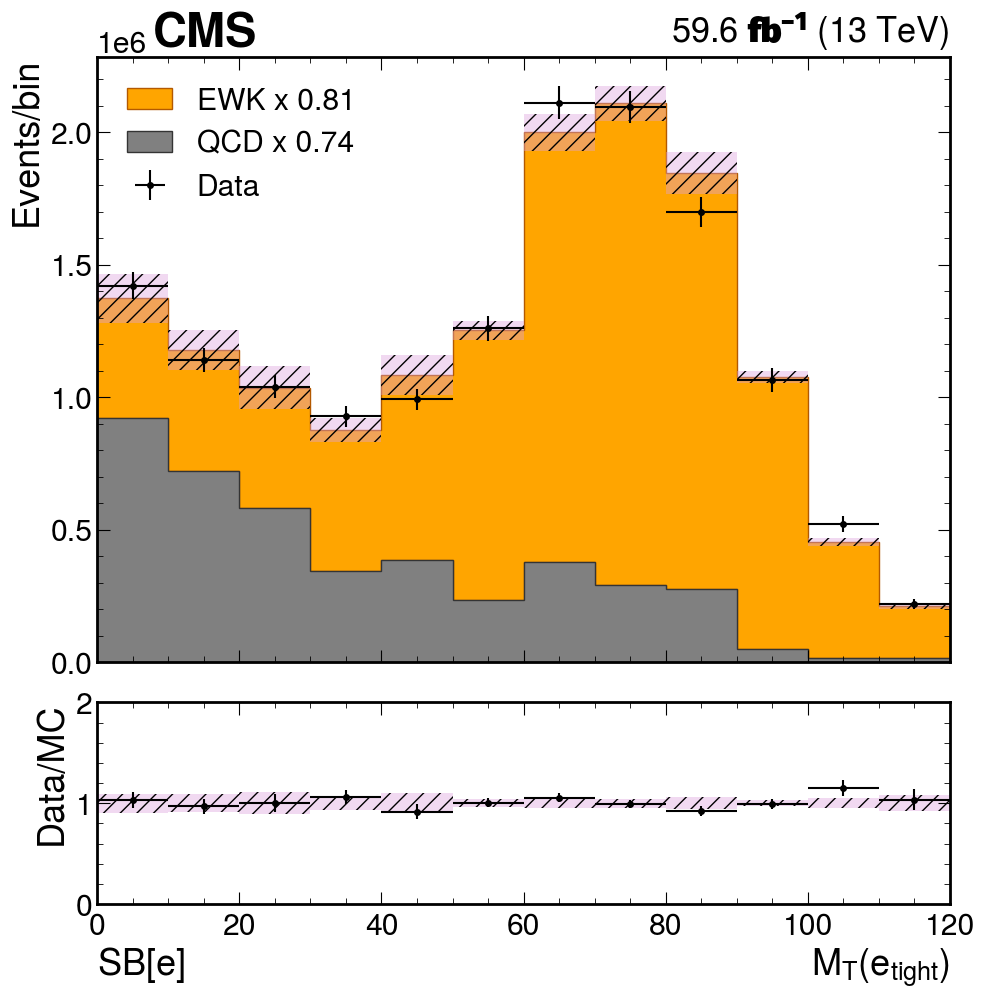
\includegraphics[width=0.35\textwidth]{template_fit/2018/mt_high_Electron_25.0.png} \hfill
  \subfigure(4) 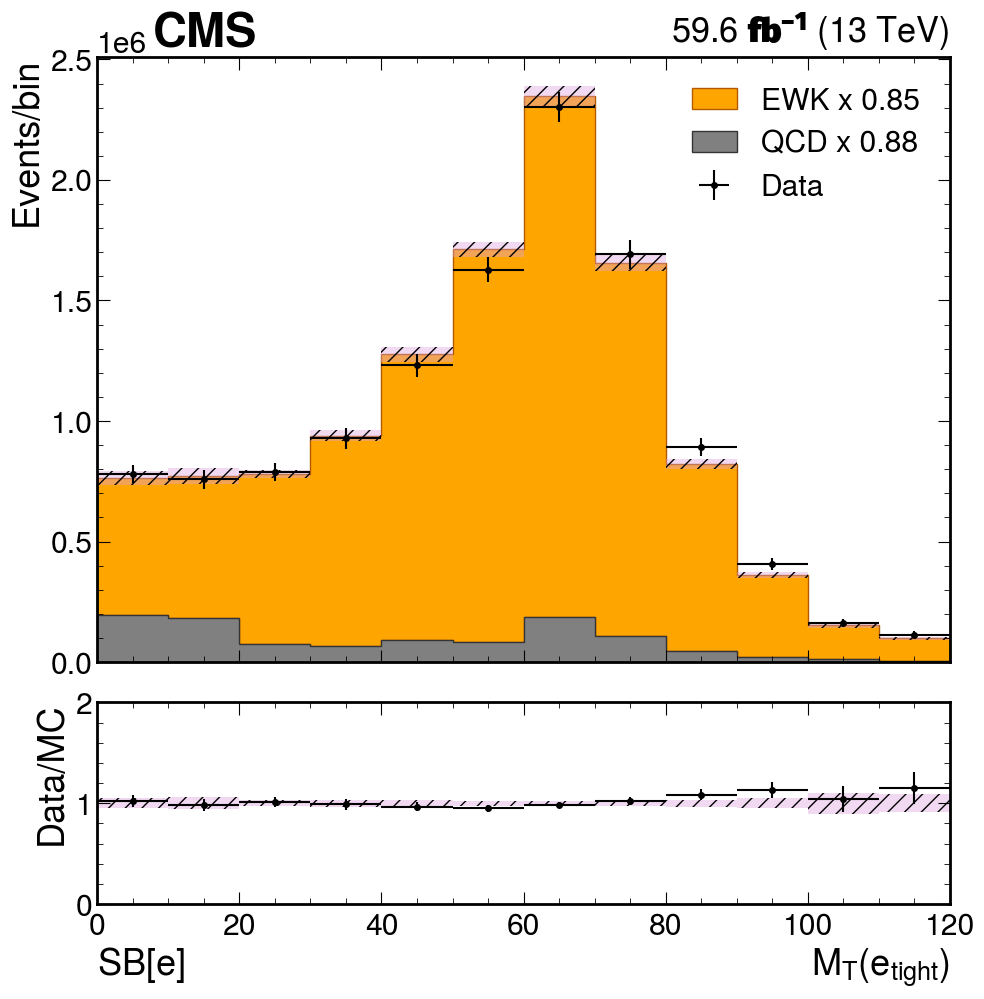
\includegraphics[width=0.35\textwidth]{template_fit/2018/mt_high_Electron_45.0.png} \\
  \subfigure(5) 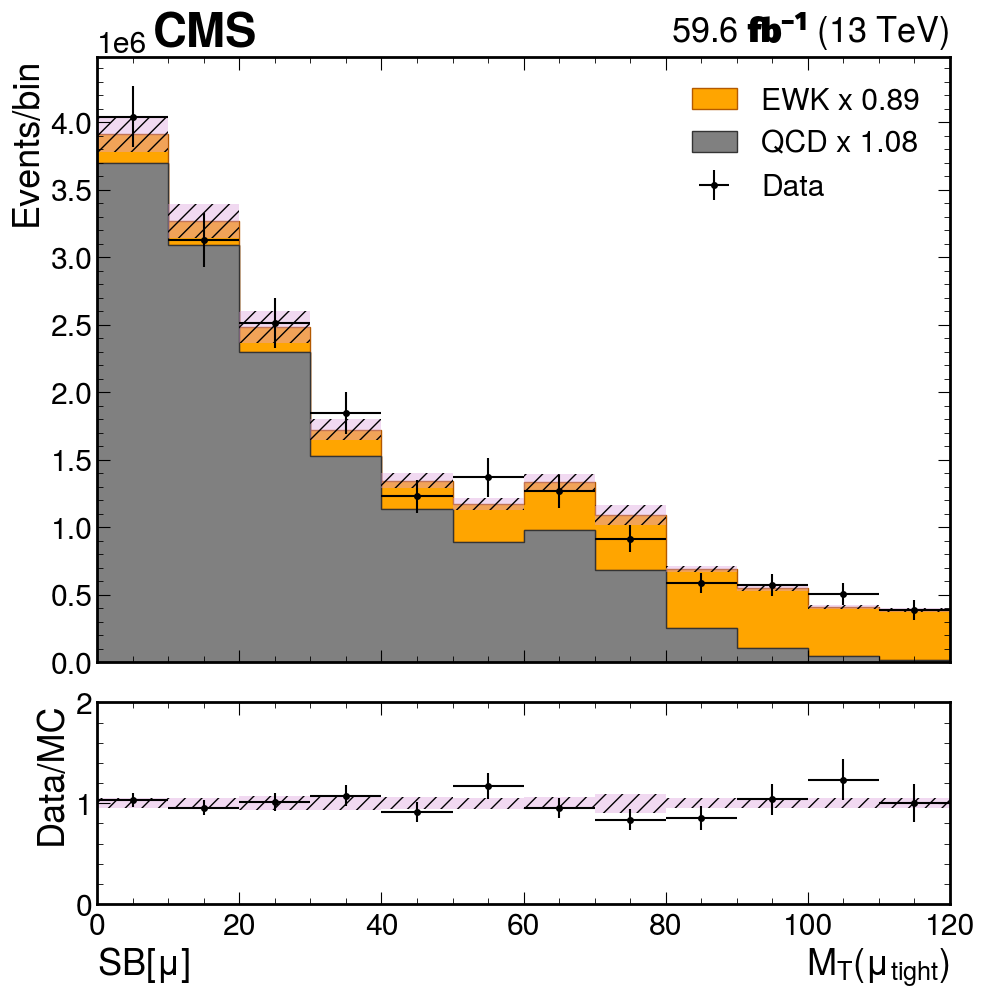
\includegraphics[width=0.35\textwidth]{template_fit/2018/mt_low_Muon_15.0.png} \hfill
  \subfigure(6) 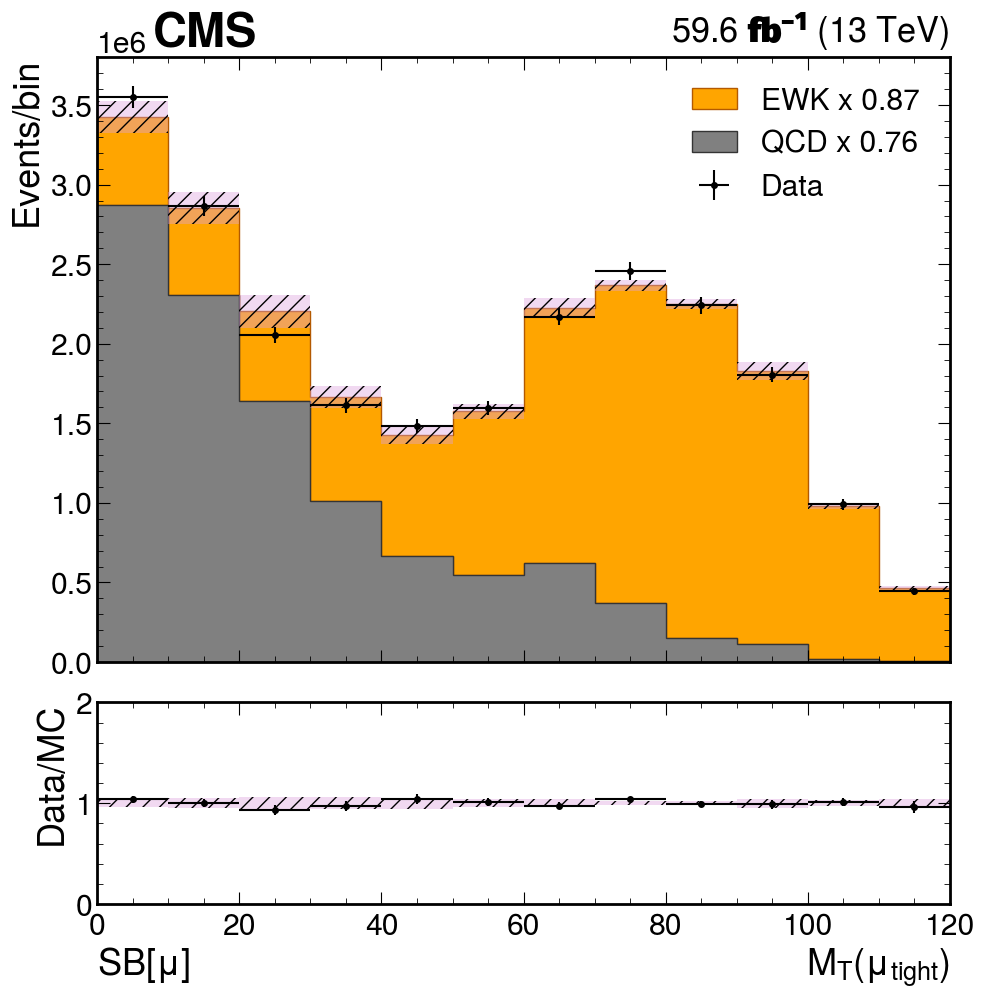
\includegraphics[width=0.35\textwidth]{template_fit/2018/mt_high_Muon_20.0.png} \\
  \subfigure(7) 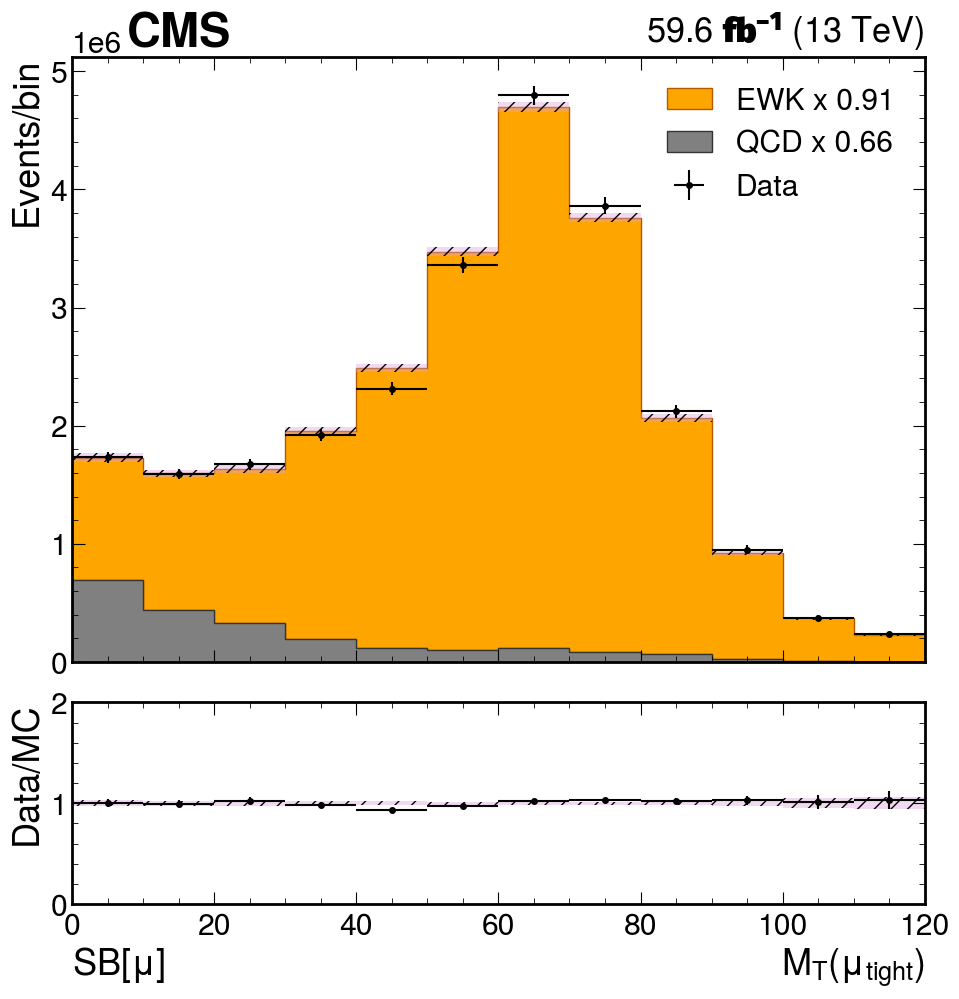
\includegraphics[width=0.35\textwidth]{template_fit/2018/mt_high_Muon_35.0.png}
  \caption{Results of the Template fit for 2018. Top 4 plots are for Electrons for the $\pt$ ranges of $\pt < 20\gev$ (1), $20\gev<\pt<25\gev$ (2), $25\gev<\pt<45\gev$ (3), and $\pt>45\gev$ (4), while the bottom 3 plots are for Muons in the $\pt$ ranges of $\pt < 20\gev$ (5), $20\gev<\pt<35\gev$ (6), and $\pt>35\gev$ (7)}
\end{figure}

\subsubsection{Measured Fake Rate}\label{sec:nonprompt:measurement}

For the Measurement of the fake rate, we choose a region enriched in QCD.\@ To accomplish this, we require $\MET$ to be low. The list of cuts applied are shown below:

\begin{itemize}
  \item Pass single Lepton trigger (trigger by $\pt$)
  \item 1 Fake/Tight Lepton
  \item $N_{j} = 1$ with $\Delta R(j, \ell) > 1$
  \item Recoiling jet passes Medium btagging WP for Muons
  \item $\MET < 30\gev$
\end{itemize}

After applying the template scale factors derived in our sideband region, we calculate the fake rate in 2 ways: using exclusively QCD MC and using data subtracting out the EWK MC.\@ The data driven fake rate is prefered, but the QCD MC allows us to cross-check our fake rates.

\begin{figure}
  \centering
  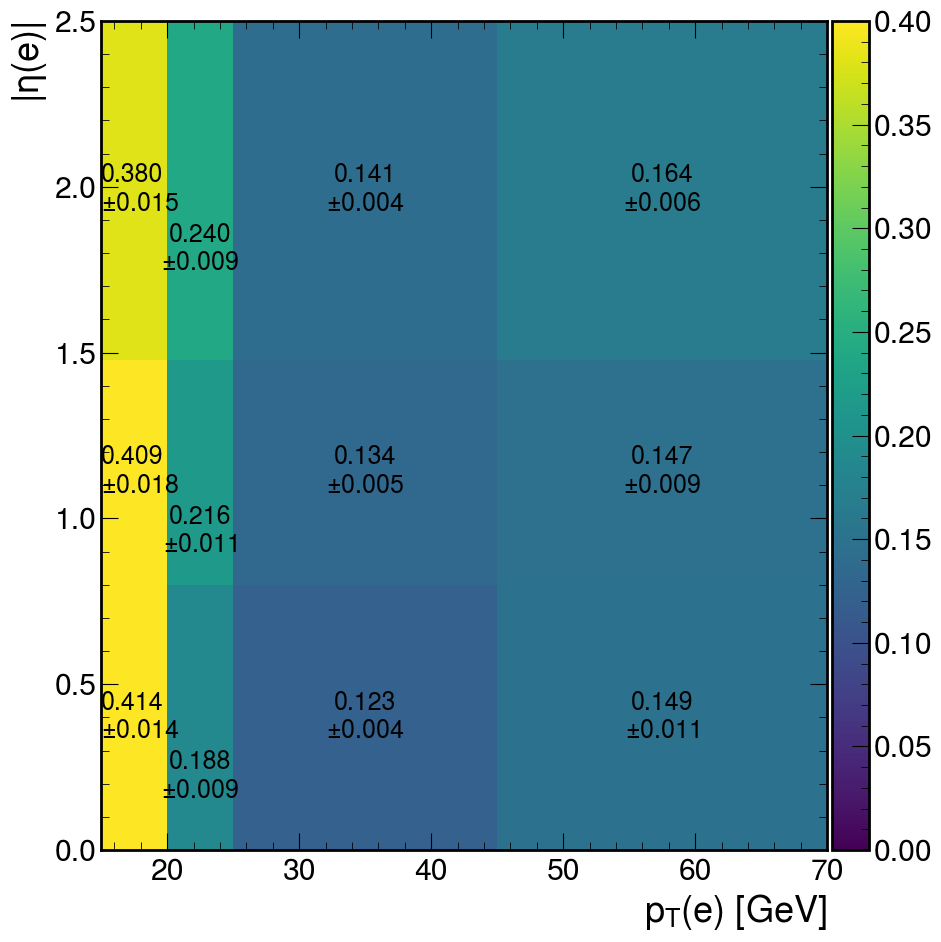
\includegraphics[width=0.45\textwidth]{measurement/2016/fr_data_ewk_Electron.png} \hfill
  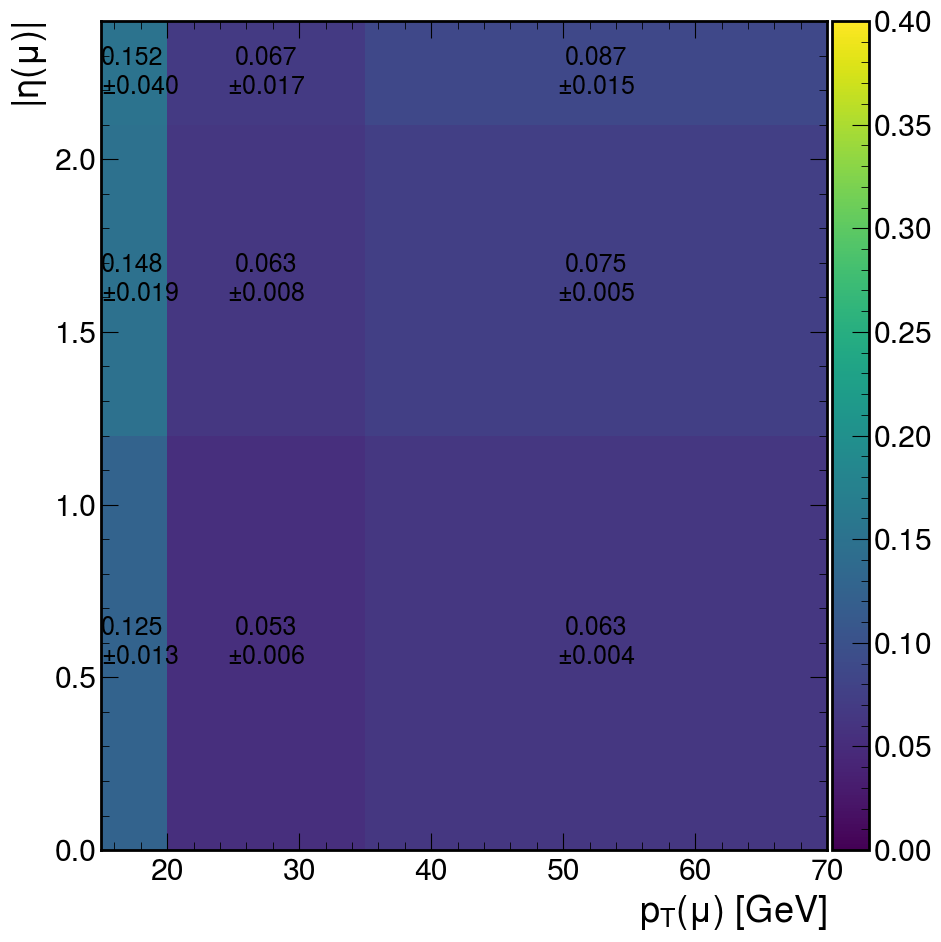
\includegraphics[width=0.45\textwidth]{measurement/2016/fr_data_ewk_Muon.png} \\
  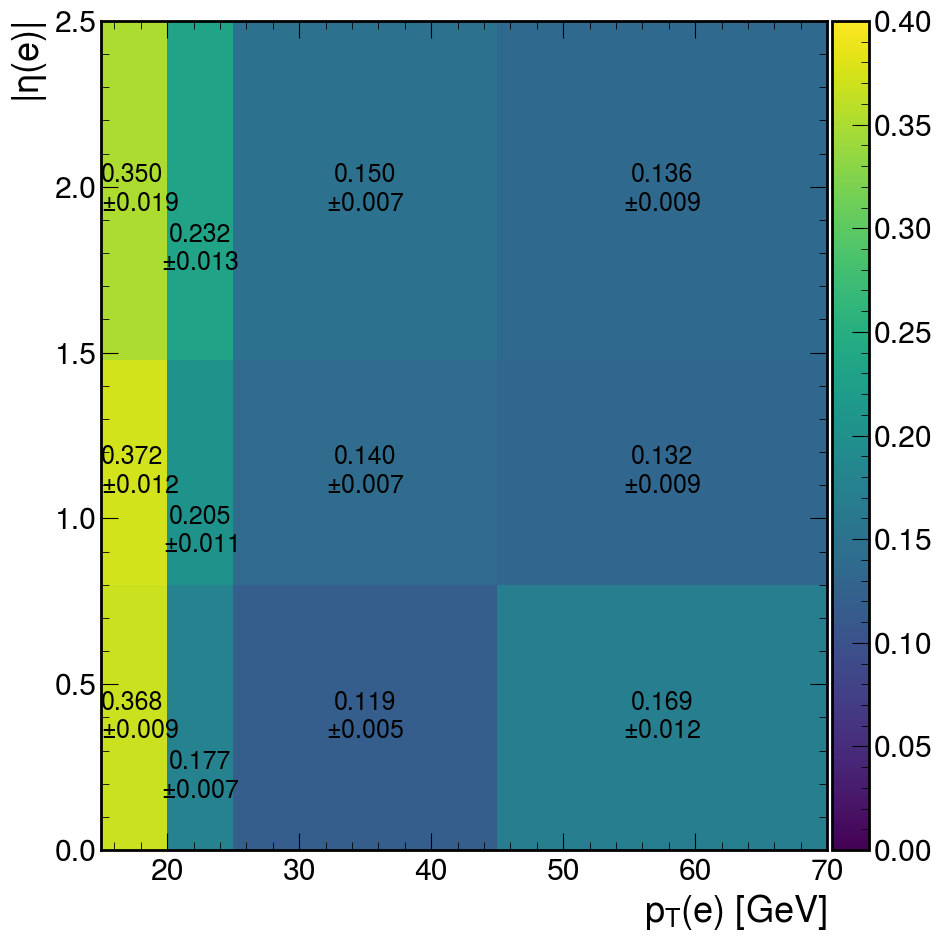
\includegraphics[width=0.45\textwidth]{measurement/2016/fr_qcd_Electron.png} \hfill
  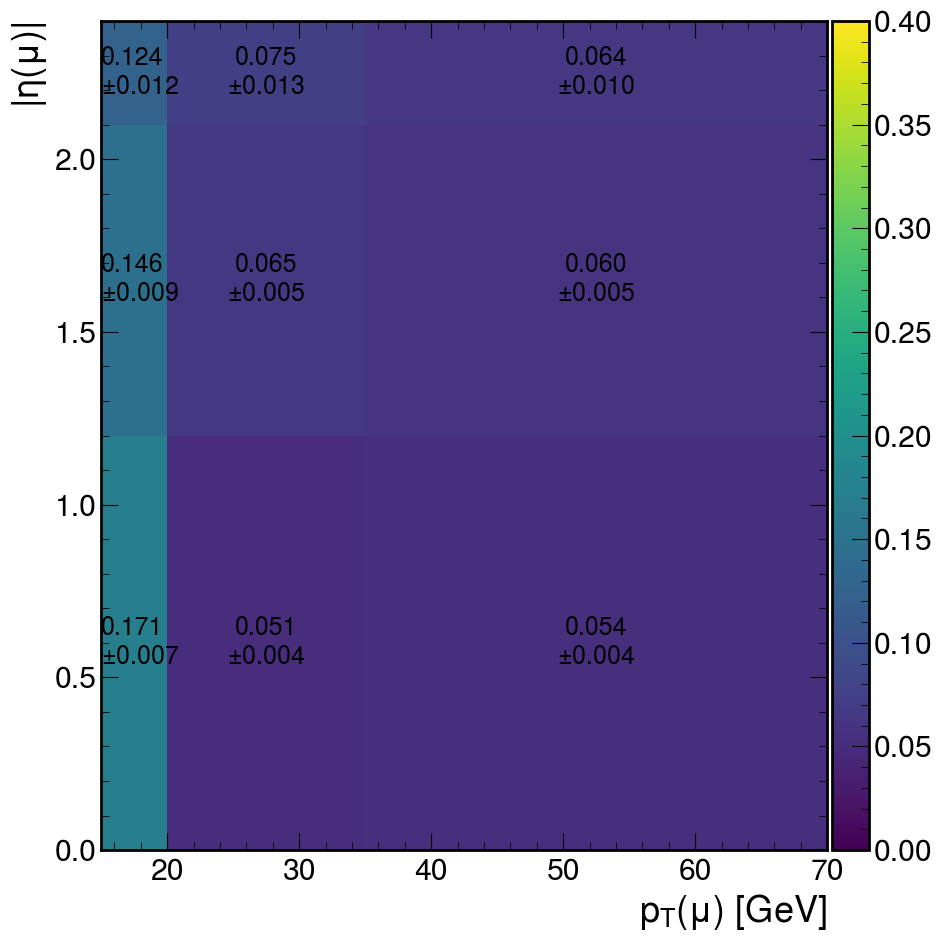
\includegraphics[width=0.45\textwidth]{measurement/2016/fr_qcd_Muon.png} \\
  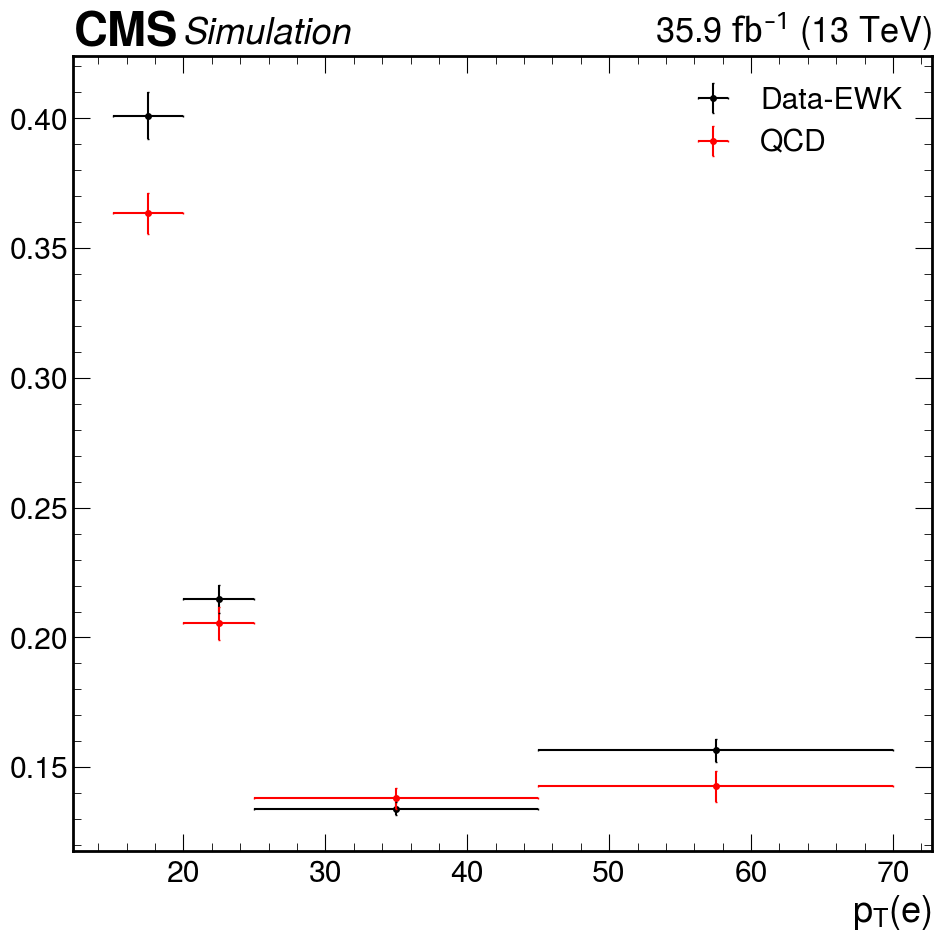
\includegraphics[width=0.45\textwidth]{measurement/2016/fr_Electron_pt.png} \hfill
  \includegraphics[width=0.45\textwidth]{measurement/2016/fr_Muon_pt.png} \\
  \caption{This shows fakes for 2016. Top row shows the fake as calculated using Data-EWK. The second row shows the fake rate as calculated using just QCD MC.\@ The last row shows a comparison of the two methods in the $\pt$ spectrum. On the left is the fake rates for Electrons while the right shows the fake rates for muon}
\end{figure}

\begin{figure}
  \centering
  \includegraphics[width=0.45\textwidth]{measurement/2017/fr_data_ewk_Electron.png} \hfill
  \includegraphics[width=0.45\textwidth]{measurement/2017/fr_data_ewk_Muon.png} \\
  \includegraphics[width=0.45\textwidth]{measurement/2017/fr_qcd_Electron.png} \hfill
  \includegraphics[width=0.45\textwidth]{measurement/2017/fr_qcd_Muon.png} \\
  \includegraphics[width=0.45\textwidth]{measurement/2017/fr_Electron_pt.png} \hfill
  \includegraphics[width=0.45\textwidth]{measurement/2017/fr_Muon_pt.png} \\
  \caption{This shows fakes for 2017. Top row shows the fake as calculated using Data-EWK. The second row shows the fake rate as calculated using just QCD MC.\@ The last row shows a comparison of the two methods in the $\pt$ spectrum. On the left is the fake rates for Electrons while the right shows the fake rates for muon}
\end{figure}

\begin{figure}
  \centering
  \includegraphics[width=0.45\textwidth]{measurement/2018/fr_data_ewk_Electron.png} \hfill
  \includegraphics[width=0.45\textwidth]{measurement/2018/fr_data_ewk_Muon.png} \\
  \includegraphics[width=0.45\textwidth]{measurement/2018/fr_qcd_Electron.png} \hfill
  \includegraphics[width=0.45\textwidth]{measurement/2018/fr_qcd_Muon.png} \\
  \includegraphics[width=0.45\textwidth]{measurement/2018/fr_Electron_pt.png} \hfill
  \includegraphics[width=0.45\textwidth]{measurement/2018/fr_Muon_pt.png} \\
  \caption{This shows fakes for 2018. Top row shows the fake as calculated using Data-EWK. The second row shows the fake rate as calculated using just QCD MC.\@ The last row shows a comparison of the two methods in the $\pt$ spectrum. On the left is the fake rates for Electrons while the right shows the fake rates for muon}
\end{figure}

\subsubsection{Closure Test}\label{sec:nonprompt:closure}

To test the fake rates measured, we do so in a signal-like closure region. Our signal region is primarily composed of a high $\HT$ and 2 same-sign leptons, but we relax these cuts to boost statistics for testing the overall agreement. The closure region cuts are listed below:

\begin{itemize}
  \item Dilepton Trigger
  \item 2 Same Sign Leptons (Fake or Tight)
  \item $M_{\ell\ell} < 12\gev$ and $|M_{Z}-M_{\ell\ell}| < 15\gev$
  \item $N_{j} \ge 1$
  \item $\HT \ge 125\gev$
  \item $\MET > 50\gev$
\end{itemize}

For applying the fake rates, we note that our fake rate is actually a ratio of Tight leptons to Fake leptons (Tight inclusive) making it a ratio of Fake leptons that are also Tight. For our application, we are transfering events from a Fake region to a Tight region, so we need the ratio of Tight leptons to Fake leptons (Tight excluded), making our weight we apply $\frac{f}{1-f}$ where f is the fake rate.

Because our signal region is a multi-lepton region, we need to also consider double counting in our application. For a 2 lepton case, we consider 3 regions: the Tight-Tight (TT), Tight-Fake (TF), and Fake-Fake (FF). For transfering events from the TF, we note that there are events with 1 nonprompt lepton and events with 2 nonprompt leptons where one of these nonprompt leptons is faking a Tight lepton. Because for the case of 2 nonprompt leptons, either could have faked being a tight lepton, we end up double counting events with 2 nonprompt leptons. To correct for this, we need to subtract these events from the FF region.

This logic can be extended to the 3 lepton case and we see an extra negative sign is needed for every even number of Fake leptons in the event, or:

\begin{equation}
  \label{eq:1}
  w = (-1)^{N_{\ell}}\prod_{i}^{N_{\ell}}\frac{f(\pt(i), \eta(i))}{1-f(\pt(i), \eta(i))}
\end{equation}

Applying these factors to our TF and FF closure regions, we get an estimation of the nonprompt background in our TT closure region. Since the nonprompt background comes from high cross-section samples that have a lepton originating from a jet faking a prompt lepton, we expect ttbar and W+Jets to dominate (Drell-Yan being removed from the Z veto). Comparing our nonprompt data-driven estimation to the MC, we see agreement is fair. Keeping in line with other analyses and the agreement in our closure region, we estimate our systematic error from the Nonprompt Fake rate being the error in the statistics of the fake rate measurement itself and a 30\% log-normal systematic coming from the agreement in our closure region.

\begin{figure}
  \centering
  \includegraphics[width=0.31\textwidth]{closure/2016/ht_TT_EE.png} \hfill
  \includegraphics[width=0.31\textwidth]{closure/2016/ht_TT_EM.png} \hfill
  \includegraphics[width=0.31\textwidth]{closure/2016/ht_TT_MM.png} \\
  \includegraphics[width=0.31\textwidth]{closure/2017/ht_TT_EE.png} \hfill
  \includegraphics[width=0.31\textwidth]{closure/2017/ht_TT_EM.png} \hfill
  \includegraphics[width=0.31\textwidth]{closure/2017/ht_TT_MM.png} \\
  \includegraphics[width=0.31\textwidth]{closure/2018/ht_TT_EE.png} \hfill
  \includegraphics[width=0.31\textwidth]{closure/2018/ht_TT_EM.png} \hfill
  \includegraphics[width=0.31\textwidth]{closure/2018/ht_TT_MM.png} \\
  \caption{Closure plots for 2016 (top), 2017 (middle), and 2018 (bottom) considering all three channels, EE (left), EM (middle), and MM (right)}\label{fig:a}
\end{figure}


\subsection{Charge Mis-Identification}\label{sec:charge_misId}
Our signal region is two same-sign leptons which removes the large ttbar and Drell-Yan samples from our yield, but this is dependent on the two leptons in samples such as ttbar and Drell-Yan having their charge identified correctly. The charge of the leptons is usually determined by the direction of the curvature of the lepton in the beam. This means that the CMS detectors' ability to measure the correct charge is dependent on the lepton's $\pt$ and $\eta$. Further, charge misId is more likely in electrons than muon because of the stochastic bremsstrahlung more prevalent in electrons.

The fake rate is measured in a signal like region using MC since there is no way to decide if a lepton's charge actually flipped or not in data. The overall fake rate is corrected by fitting the normalization based on the closure plot to account for the difference in simulated and actual charge misId. The closure is done in a Drell-Yan enriched region in the same-sign region with events transferred from the opposite-sign region.

The measurement region cuts are listed below:

\begin{itemize}
  \item Trigger requirements
  \item 2 Tight Leptons with Lepton Veto
  \item $M_{\ell\ell} > 50\gev$
  \item $N_{j} \ge 2$
  \item $H_{T} > 100\gev$
  \item $\MET > 25\gev$
\end{itemize}

The closure region cuts are listed below:

\begin{itemize}
  \item Trigger requirements
  \item 2 opposite-sign Tight Electrons with Lepton Veto
  \item $70\gev < M_{ee} < 115\gev$
  \item $H_{T} < 250\gev$
  \item $\MET < 50\gev$
\end{itemize}

% \end{document}

%%% Local Variables:
%%% mode: latex
%%% TeX-output-dir: "build"
%%% TeX-master: "../AN"
%%% End:
